\documentclass{report}
\usepackage{parskip}
\setlength{\parindent}{15pt}
\usepackage[utf8]{inputenc}
\usepackage[left=2.5cm,right=2.5cm,top=3cm,bottom=3cm]{geometry}
%\usepackage{natbib}
\usepackage{graphicx}
\usepackage{amsmath}
% \usepackage{wrapfig}
\usepackage{fancyhdr}
\usepackage{fancyvrb}
\usepackage{titlesec}
\setcounter{secnumdepth}{4}
% \renewcommand{\baselinestretch}{0.0}
\usepackage{indentfirst}
\usepackage{mathtools, nccmath}
\usepackage[export]{adjustbox}
\usepackage[caption=false, font=footnotesize]{subfig}
\usepackage{verbatim}
\pagestyle{fancy}
\fancyhf{}
%\rhead{Intelligent System}
%\lhead{M1MoSIG}
\rfoot{\thepage}
\titleformat{\paragraph}[hang]{\normalfont\normalsize\bfseries}{\theparagraph}{1em}{}
\titlespacing*{\paragraph}{0pt}{2ex plus 1ex minus .2ex}{0.5em}

%\title{\textbf{Exercise\smallbreak Recognizing Digits using Neural Networks}}
%\author{Group 11: Dinh Khoa TRAN - Sebastien RIOU - Maxime CALKA}
%\date{March 2018}



\begin{document}
\begin{titlepage}

\begin{minipage}{0.47\textwidth}

\includegraphics[width=0.8\textwidth, left]{UPMC_Sorbonne_logo.png}
\end{minipage}
\begin{minipage}{0.47\textwidth}

\includegraphics[width=0.8\textwidth, right]{EURECOM_logo.jpg}
\end{minipage}
\par\vspace{1cm}
\centering
{\scshape\Large First year report\par}
\par\vspace{1cm}

   \begin{center}
       \vspace*{1cm}
        \Huge
       \textbf{Ultra-Reliable Low-Latency Communications in 5G }
 
       \vspace{0.5cm}
       \Large
        PHY design in Ultra-Reliable Low-Latency Communications 
 
       \vspace{1.5cm}
 
       \textbf{LE Trung Kien}\\
       \textbf{Professor: Florian KALTENBERGER}
 
       \vfill
 

 
       \vspace{0.8cm}
 

       %\includegraphics[width=0.4\textwidth]{university}
       
       %TCT Mobile Europe SAS and EURECOM\\
       
      {\large \today\par}
 
   \end{center}
\end{titlepage}
%\maketitle

\thispagestyle{fancy}
\tableofcontents{}
\clearpage

\chapter{Introduction}
\section{NR overview}
\begin{figure}[htbp]
\centerline{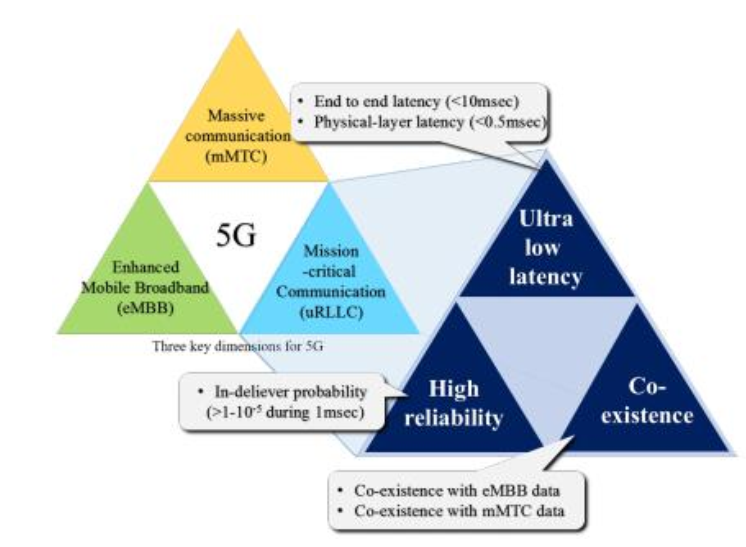
\includegraphics[scale=0.35]{fig29.PNG}}
\caption{Service categories and requirements of 5G NR.}
\label{fig29}
\end{figure}

The emergence of new paradigms like connected self-driving cars, automated industrial control, augmented and virtual reality led the wireless standardization bodies to take these into account. To that respect, 3GPP has defined three service paradigms for 5G: Enhanced Mobile Broadband (eMBB), Massive Machine-Type Communication (mMTC) and Ultra-Reliable Low Latency Communication (URLLC).

eMBB targets high data rate transmission with high requirements for bandwidth such as virtual reality, real time security, 3-dimensional image and 4K-resolution video streaming. The goal in NR design is to increase system throughput.

mMTC aims to support a large number of low-power devices for a long life-time requiring highly energy efficient communication. They demand the improvements of latency, reliability, massive connection density and energy efficiency. 
 
URLLC is for devices requiring low latency and high link reliability such as autonomous vehicle, remote surgery in medical field and industrial autonomation. They are real time applications that require the immediate actions so time requirement is very strict being in the order of ten-hundreds of microseconds. 

Among these three service categories, URLLC raises the most challenge because it has to deal with two requirements that have trade-off: reliability and latency. Basically, one of two factors must be sacrificed to attain the other factor. 

In \cite{ad1}, The 3rd Generation Partnership Project (3GPP) defines targets for the URLLC scenario: ``A general URLLC reliability requirement for one transmission of a packet is 10\textsuperscript{-5} for 32 bytes with a user plane latency of 1 ms''. The next release of 3GPP will have higher requirements of URLLC: ``Higher reliability (up to 10\textsuperscript{-6}), higher availability, short latency in the order of 0.5 to 1 ms, depending on the use cases (factory automation, transport industry and electrical power distribution)''\cite{ad2}.

\section{Techniques standardized by 3GPP in URLLC design}

In order to achieve URLLC requirements, some principal techniques are specified in 3GPP Release 15 finalized in December 2018.

The first aspect is related to the usage of flexible sub-carrier spacing (SCS). In LTE, the value of SCS is fixed at 15 kHz. In contrast, as shown in Fig.~\ref{fig32},  the value of SCS in 5G can be 15 kHz, 30 kHz, 60 kHz, 120 kHz and 240 kHz \cite{ad6}. This results in shorter symbols and slots. As data is normally scheduled at slot level, the network becomes very reactive to uplink (UL) and downlink (DL) traffic demands. Thus, the time alignment and transmission of packets becomes much faster compared to that of LTE.

\begin{figure}[htbp]
\centerline{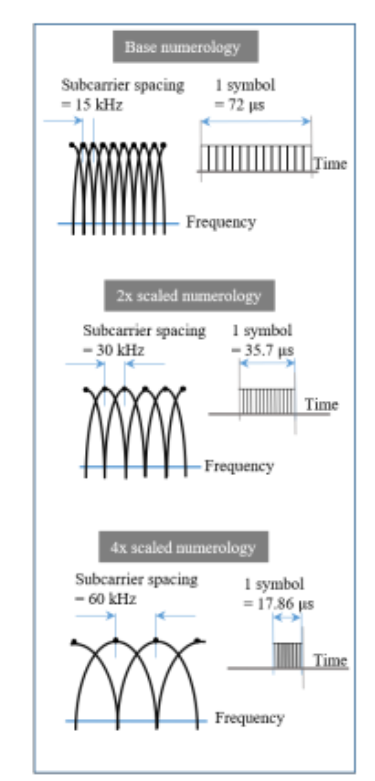
\includegraphics[scale=0.35]{fig32.png}}
\caption{Numerologies in 5G NR.}
\label{fig32}
\end{figure}

The second aspect is related to mini-slot based transmissions as shown in Fig.~\ref{fig33}. It has been agreed that a packet can be scheduled to be transmitted in DL or UL in the interval of one or several symbols instead of the whole slot as LTE \cite{ad7}.

\begin{figure}[htbp]
\centerline{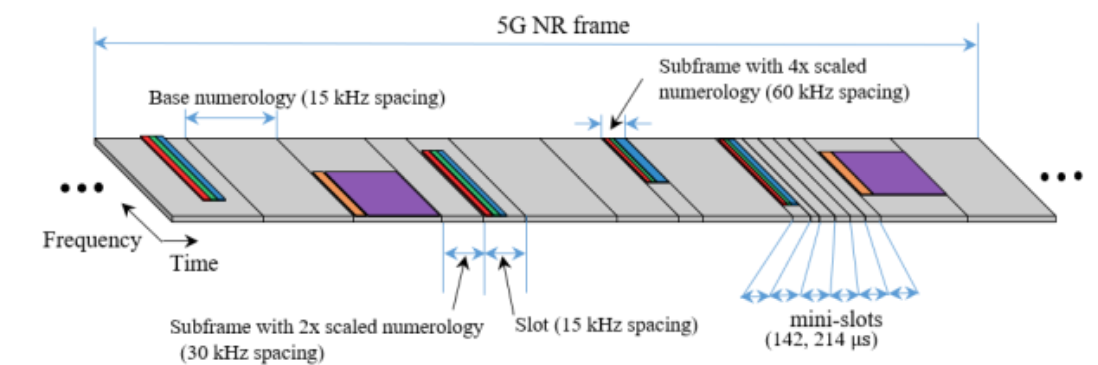
\includegraphics[scale=0.35]{fig33.png}}
\caption{Frame structure in 5G NR.}
\label{fig33}
\end{figure}

The third aspect is the standardization of the UL configured grant (CG) transmissions. In the conventional grant-based (GB) transmission, when a user equipment (UE) has data to transmit, it must send scheduling request (SR) to the base station (gNB) then receives UL grant from the gNB for UL resource allocation. However, in a CG transmission, the UE is configured with the periodic transmission resources by the gNB so it can transmit data immediately in these resources without the presence of SR and UL grant \cite{ad3}. This transmission mode helps to reduce the processing and transmission time of SR and UL grant that brings significant latency advantage to UL transmission.

A fourth aspect is the flexible configurable HARQ timing. Contrary to the fixed duration of 4 milliseconds between data transmission and its associated HARQ response in LTE, 5G allows flexible configuration of HARQ timing, even permitting the same slot HARQ response for some low latency applications \cite{ad23}.

These new features have allowed achieving significantly large quality of service (QoS) requirements compared to what was possible with 4G. Yet, the URLLC applications described previously may still benefit with improved link performance. 3GPP Release-16, currently under standardization, is trying to make further progress on some important topics such as PDCCH reliability, PUSCH enhancements, eMBB and URLLC multiplexing, and UL CG enhancements etc. 

\section{Main contribution}

This work contributes to solve two major problems relevant to URLLC, acknowledged by 3GPP. Chapter \ref{S2} deals with the first problem of URLLC performance's deterioration in eMBB and URLLC multiplexing in UL CG transmission. This section summarizes the method related to two-step strategy with overlap indication and explicit feedback structure or an additional SR that is presented and published in  PIMRC 2019 paper "Improving Ultra-Reliable Low-Latency Communication in multiplexing with Enhanced Mobile Broadband in grant-free resources" \cite{ad99}. It is also filed in the patent: "Uplink multiplexing in cellular wireless communication networks (application number: 1820784.5). 

Chapter \ref{S3} copes with another important problem of URLLC related to less-than-K-repetitions UL CG transmissions. These UEs may be configured with CG transmissions frequently to avoid scheduling delays, and with multiple repetitions for the same transport block (TB) to ensure a certain reliability. As packet arrival at the UEs is not aligned to system timing, packets appearing in the middle of the interval will either have to wait for the next interval to transmit the configured number of repetitions or transmit fewer repetitions in the current interval. The former may be a problem for latency whereas the latter may lead to reliability issue. Three different techniques to solve this problem or at least alleviate the harmful effect of a smaller number of repetitions transmitted that we proposed in \cite{b9} and \cite{ad100} are described and compared with each other. The first technique in Section \ref{32} published in EuCNC 2019 paper "Optimal reserved resources to ensure the repetitions in Ultra-Reliable Low-Latency Communication Uplink Grant-free transmission" \cite{b9} uses reserved resources so that the UE can use them to transmit the repetitions until it reaches the configured number. The sizes of the reserved resources are optimized based on their positions. The second technique in Section \ref{331} demands the UE to activate explicit HARQ feedback structure if it cannot do all repetitions as configured. This structure helps reduce the probability of packet loss due to DMRS miss-detection. The third technique in Section \ref{332} asks the UE to transmit an additional SR in case of a smaller number of repetitions transmitted. This SR provides another chance for the gNB to recognize UE appearance so that packet loss's probability decreases. The second and third methods are published in ISWCS 2019 paper "Strategies to meet the configured repetitions in URLLC Uplink Grant-Free transmission" and are filed in the patent: "Uplink HARQ in cellular wireless communication networks" (application number: 1821058.3). 

Chapter \ref{S4} discuss the future works for the next years. Chapter \ref{S5} concludes the works and lists the achievements of the first year.


\chapter{Strategies in Enhanced Mobile Broadband and Utra-Reliable Low-Latency Communication multiplexing in configured grant resources} \label{S2}

\section{Problem formulation}

In 5G New Radio (NR),  in order to reduce the time consumption of scheduling request (SR) and uplink (UL) grant, the base station (called gNB) can configure a set of configure-grant (CG) resources to one or more users (UEs) with a periodicity defined by parameters in RRC from higher layer \cite{ad3}. When a UE is configured to transmit in CG resources, it can transmit data immediately instead of sending SR and waiting for UL Grant as grant-based (GB) transmission. However, the gNB does not have any prior information which of these CG resources will actually be used by URLLC UEs or which of the UEs in the group configured to the resources will use a specific resource. If the cell is loaded and the gNB schedules some eMBB UEs on the resource overlapping with CG occasion, as shown in Fig.~\ref{fig1}, there is going to be transmission collision of dynamically scheduled eMBB and URLLC CG transmissions. 

\begin{figure}[htbp]
\centerline{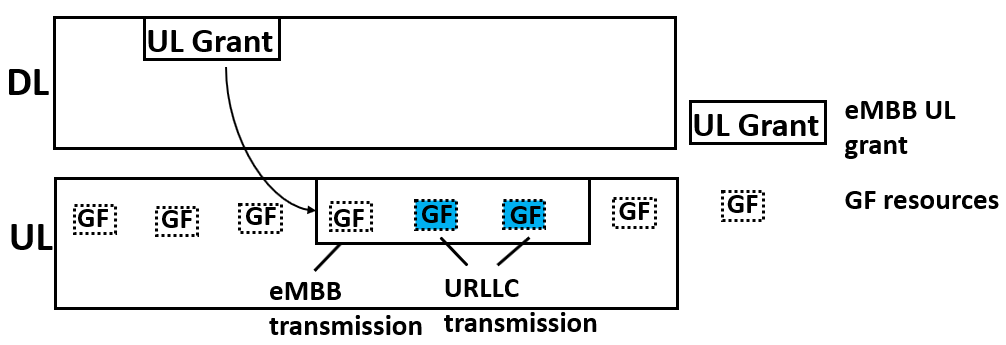
\includegraphics[scale=0.3]{fig1.PNG}}
\caption{A collision of UL URLLC CG transmission with eMBB transmission in case of Frequency Division Duplex (FDD).}
\label{fig1}
\end{figure}

When the transmissions from eMBB and URLLC UEs in CG resources overlap, it results in lower decoding probability due to lower resulting SINR for both UEs. This can be a serious problem for URLLC UEs in particular due to their tight latency and reliability targets.

\section{Mechanism to support preemption indication}\label{22}
To avoid a collision between eMBB and URLLC transmission, preemption indication (PI) is transmitted by the gNB to stop the eMBB transmission in the overlapping region. URLLC transmission is mini-slot transmission. Thereby, in case PI is transmitted to the eMBB UEs, it must be done in mini-slot level to be likely to stop the transmission in time and satisfy the traffic critical delay. This design requires that the eMBB UEs monitor PI in mini-slot level. However, the eMBB UEs transmit data in slot level and also only monitors DCI in slot level. This means that if DCI is used as PI, the eMMB UEs are required to increase monitoring periodicity. Monitoring capability of the eMBB UEs also must be enhanced with a growth of monitoring occasions. A mechanism to select the eMBB UEs and trigger an increase of monitoring periodicity and capability is necessary.

\subsection{Selection of the eMBB UEs monitoring PI in mini-slot level} \label{221}
In semi-static resource sharing, there are the regions that are exclusive to eMBB or URLLC transmissions. Because URLLC traffic might be sparse, the eMBB UEs are able to be configured to transmit in one part of URLLC band. This band is called a shared/co-existence region. When the eMBB UEs are allocated transmission resource in the only-eMBB band, it is certain that there is no collision with the URLLC UEs. Thereby, the gNB does not need to activate these UEs to increase monitoring periodicity in order to listen to PI. In contrast, if the eMBB UEs are configured to transmit in the shared region, there is a chance that the gNB must stop their transmission to prioritize URLLC transmission. These eMBB UEs are required to listen to PI in mini-slot level so that they can stop their transmission in the shortest delay.

In multiplexing between eMBB GB and URLLC GB transmission, only the eMBB UEs that are chosen as candidates for potential cancellation by the gNB are triggered to increase monitoring periodicity. The eMBB UE candidates are chosen based on selection criteria following the order: UE capability, UE position to the gNB, data size and channel condition.

In multiplexing between eMBB GB and URLLC CG transmission, the eMBB UEs are triggered by the gNB to increase monitoring periodicity

\subsection{Mechanism to activate an increase of monitoring periodicity} \label{222}
If the eMBB UEs are configured to monitor PI in mini-slot level all the time after being scheduled, power consumption would rise significantly. Therefore, only the eMBB UEs specified in Section \ref{221} are triggered to increase monitoring periodicity. This activation is done by the gNB when it includes 1-bit flag in the UL grant to help the eMBB UEs perceive their situation and do monitoring in mini-slot level. The bit used as a flag can be a padding bit or the first bit in the field of frequency domain resource assignment.

\subsection{Limit of monitoring periodicity for eMBB UEs}
When an eMBB UE is indicated to decode sub-slot level pre-emption indication, it can be configured to DCI monitoring periodicity going up to its highest capability sub-carrier spacing slot timing. As an example, if a UE is capable of operating at 120 KHz SCS, and is currently operating at 15 KHz SCS, it can be configured to decode pre-emption indication DCI upto 120/15 = 8 distinct time occasions within a slot.

Monitoring capability also have to be enhanced if monitoring occasions increases. Thus, the maximum number of CCEs should be kept the same at a value to guarantee mini-slot monitoring for all SCS after the eMBB UE receives an indication by 1 bit-flag in UL grant to monitor PI in mini-slot level.

The proposals related to supporting mechanism for PI is filed in patent "eMBB and URLLC multiplexing and preemption strategies" (application number: 62790641). 

\section{Two-step strategy in multiplexing}\label{23}
\subsection{DMRS miss-detection in multiplexing}

When the transmissions from eMBB and URLLC UEs in CG resources overlap, it results in lower decoding probability due to lower resulting SINR for both UEs. This can be a serious problem for URLLC UEs in particular due to their tight latency and reliability targets.

In case the gNB is able to identify the URLLC UE from its Demodulation Reference Signal (DMRS) sequence, it may try to quickly reschedule the UE over non-overlapping resources if an error happens.

The increased interference due to overlapping transmissions of eMBB and URLLC UEs may lead to a catastrophic situation when the gNB may not even identify the URLLC UE (DMRS miss-detection). The current Hybrid automatic repeat request (HARQ) structure in UL transmission for NR is timer based, which means that upon transmission of packet, the UE will start the HARQ timer. If it receives an UL grant for the re-transmission of the same transport block (TB) from the gNB, it does the retransmission over the resources scheduled in the UL grant. If it receives no UL grant from the gNB and the HARQ timer expires, it considers that the TB was successfully decoded at the gNB and discards the data in the buffer. 

The timer-based HARQ feedback and UL GB retransmission are standardized because this minimizes the control overhead for sending HARQ feedback. This is reasonable in general but in the cases of dynamic UL multiplexing, giving rise to overlapping transmissions with CG UEs, when the gNB will not be able to identify the UEs transmitting on CG resources, the UEs will discard their packets and consider the successful detection that leads to serious performance degradation for URLLC UEs.

\subsection{Overlap indication and explicit HARQ acknowledgement (ACK) feedback}\label{232}

This paper proposes two-step strategy to overcome the problem of the multiplexed UL eMBB and URLLC transmissions. In the first step, upon scheduling a GB transmission of the eMBB UE over the CG resources, the gNB sends an indication of resource overlap to the URLLC UEs. As the gNB does not know which of the URLLC UEs configured for CG resources may become active in the current interval, this indication needs to be sent to all UEs who have been configured with the CG resources in the overlapping interval as illustrated in Fig.~\ref{fig9}. Upon receiving this overlap indication, the URLLC UEs are aware of the resources which have been dynamically scheduled for other UEs and in case of transmission,  their transmissions will be received with an increased interference.

\begin{figure}[htbp]
\centerline{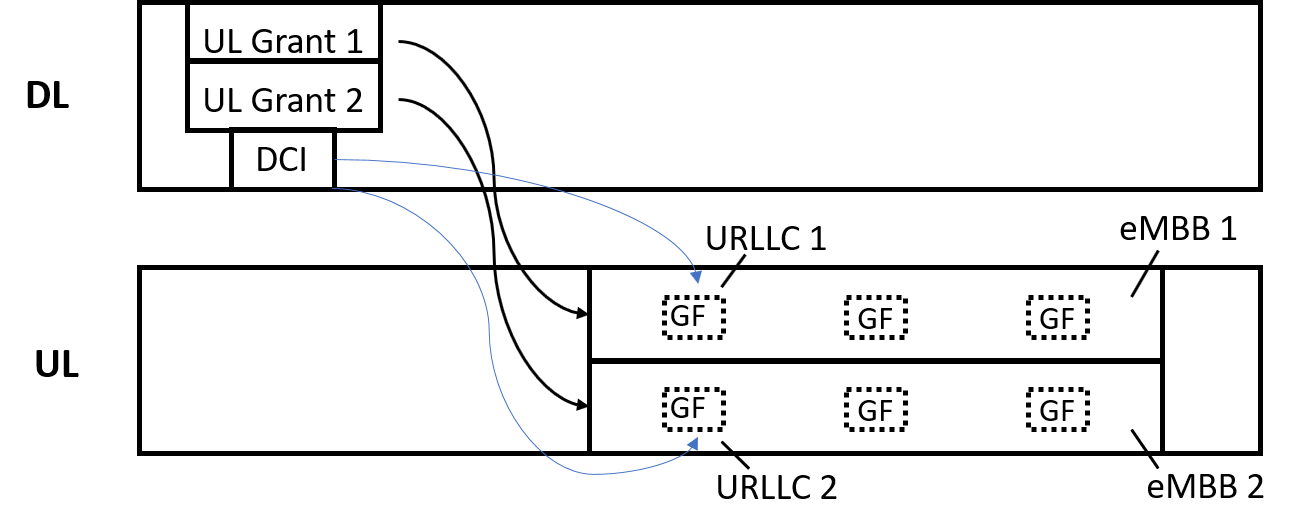
\includegraphics[scale=0.35]{fig9.png}}
\caption{Signalling the URLLC UEs about an overlap with the eMBB UEs in CG regions.}
\label{fig9}
\end{figure}

The second step of the proposed strategy comprises of making the overlapping transmissions use explicit HARQ feedback structure rather than legacy timer-based feedback. The resource overlap indication can serve this purpose by containing a 1-bit flag to tell if the feedback becomes explicit or not. Upon receiving this indication, the URLLC UEs, who transmit on the overlapping resources, expect to receive explicit HARQ feedback from the gNB for their transmissions. 

Thereby, within a configured time period, the CG UEs receive either explicit HARQ ACK indicating the successful detection of their TB or UL grant for re-transmission in case the gNB failed to decode the TB but was able to identify the transmitting UE.  For the third case, if the gNB even fails to identify the UE due to high interference (DMRS miss-detection), it cannot schedule the UE for a re-transmission in the conventional timer-based feedback so the UE assumes that a packet is decoded correctly and drops it from buffer to transmit the next packet. This is the scenario where our proposed explicit HARQ feedback becomes the most promising. If the CG UE receives neither an ACK nor an UL grant within a configured time, the UE does not consider that its data is successful, rather it considers that the gNB failed to identify its identity (ID) due to high interference in the overlapping transmissions and retransmits the TB on the subsequent CG resources. 

\subsection{Overlap indication and additional SR}

In a variation of the proposed scheme in Section \ref{232}, the second step of making the transmissions explicit HARQ feedback-based can be replaced to use an additional SR. The gNB can indicate the URLLC CG UEs by overlap indication in the first step described in Section \ref{232} to send a SR in parallel for the TB transmitted over the overlapping CG resources. The SR sent to the gNB will provide a further means besides DMRS detection to detect the ID of the UE transmitting in the interfered CG transmission. When the gNB is unable to identify the UE making the CG transmission because of DMRS miss-detection, the gNB still can identify that UE by decoding the additional SR and react fast to the received SR by sending an UL grant to this UE. Thanks to the UL grant, the UE is likely to retransmit the packet and has a successful transmission in latency budget instead of assuming a succesful transmission and dropping the packet as in the conventional scheme. When the gNB is able to decode the data successfully, it still reacts to SR to send some indications to the UE about the successful detection.

\subsection{Numerical results and performance evaluation}

\begin{table}[htbp]
\caption{Simulation parameters}
\begin{center}
\begin{tabular}{|p{8em}|p{8em}|}
 \hline
 \textbf{Parameters} & \textbf{Values}\\
 \hline
 Waveform & CP-OFDM\\
 \hline
 Subcarrier spacing & 60kHz\\
 \hline
 Channel model & Rician\\
 \hline
 K factor & 1\\
 \hline
 Number of allocated PRB & 8\\
 \hline
 DMRS detection mechanism & Time-domain correlation\\
 

%  increase row height, number of & = number of collumn
% &&&&&\\[-1em]
 
 \hline
\end{tabular}
\label{tab1}
\end{center}
\end{table}

\begin{figure}[htbp]
\centerline{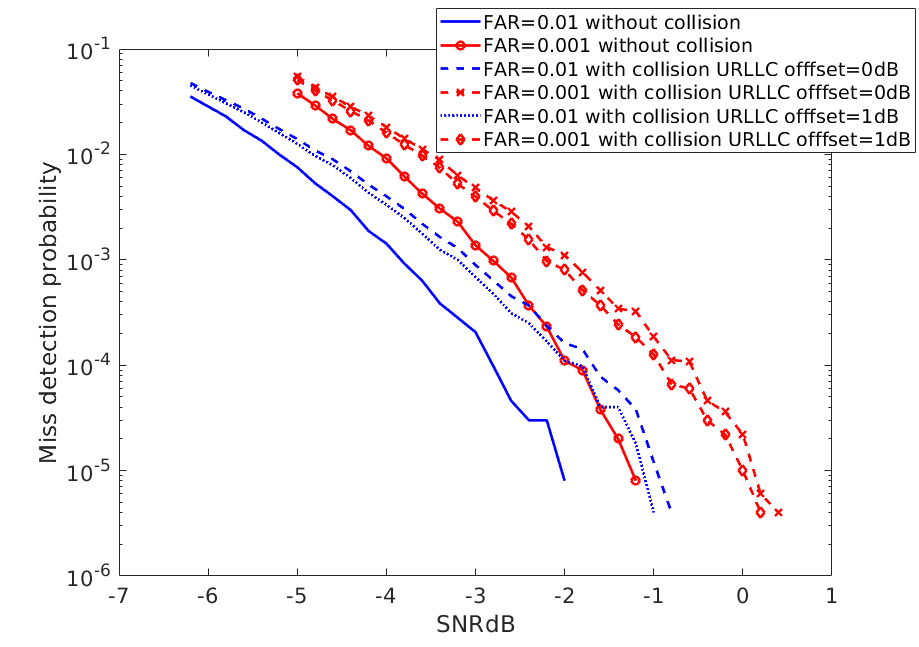
\includegraphics[scale=0.33]{fig10.png}}
\caption{DMRS detection performance.}
\label{fig10}
\end{figure}

Simulation parameters are shown in Table~\ref{tab1}. Fig.~\ref{fig10} illustrates the performance of DMRS detection in three cases: the URLLC UE transmits in the CG resources without any collision with another eMBB UE, the URLLC UE has a collision with an eMBB UE at the same power level and the URLLC UE has a collision when increasing power 1dB higher than an eMBB UE. For each DMRS detection, the correlation result is compared with a threshold to determine whether DMRS exists or not. This threshold is chosen according to a target false alarm rate (FAR) indicating the cases that the gNB determines the existence of DMRS while in reality there is no DMRS transmitted. A higher threshold is required for a lower FAR but also results in more missed detection.

Due to a collision between DMRS of the URLLC UE of interest and data/DMRS of another eMBB UE, the performance of DMRS detection of the URLLC UE degrades significantly as can be seen in Fig.~\ref{fig10} and cannot achieve the miss detection probability 10\textsuperscript{-5} at the same SNR level of the case without collision. At FAR of 0.001 and SNR of -1.4dB, the miss detection probability increases from 10\textsuperscript{-5} of the case without collision to 3.4$\times$10\textsuperscript{-4} of the case with a collision with an eMBB UE at the same power. Fig.~\ref{fig10} also shows that even with power control scheme in \cite{ad4} and \cite{ad5} when the URLLC UE's power increases 1dB higher than the eMBB UE's power, miss detection probability is still 2.44$\times$10\textsuperscript{-4} that is higher than 10\textsuperscript{-5} of the case without collision. As DMRS dectection is mandatory for channel estimation to decode data as well as for recognizing UE ID to reschedule a retransmission if necessary in conventional scheme, a degradation of DMRS detection makes the system unable to support reliability URLLC requirement. BLER of an UL transmission with one potential retransmission in the conventional scheme or power control scheme ($ P^{e}_{1}$) is calculated as\useshortskip

\begin{equation}
\begin{split}
 &P^{e}_{1} = P^{e}_{DMRS1} + \\
        &+ (1-P^{e}_{DMRS1})P^{e}_{d1}(P^{e}_{DMRS2} + (1-P^{e}_{DMRS2})P^{e}_{d2}),\label{eq1}   
\end{split}
\end{equation}
where $ P^{e}_{DMRS1}, P^{e}_{DMRS2}$ are the miss detection probabilities of the initial (with collision) and retransmitted (without collision) DMRS (see Figure \ref{fig10}), and $P^{e}_{d1}, P^{e}_{d2}$ are the error probabilities of the initial (with collision) and retransmitted (without collision) PUSCH.

In \eqref{eq1}, the first term is the error probability when the gNB cannot detect DMRS to decode or reschedule data so the UE does not retransmit data and data is lost. The second term is the error probability when the gNB detects DMRS and indentifies UE ID but fails to decode data so it reschedules data. However, it cannot decode the retransmission and an error still occurs.

The usage of an explicit HARQ feedback as explained in Section \ref{232} solves the problem of DMRS miss-detection in the overlapping region because it allows the UE to carry out the retransmissions in the interference-free regions even if DMRS is not detected by the gNB. BLER of an UL transmission with one potential retransmission in the proposed scheme with explicit feedback ($ P^{e}_{2}$) is calculated as\useshortskip

\begin{equation}
\begin{split}
 &P^{e}_{2} = P^{e}_{DMRS1}(P^{e}_{DMRS2} + (1-P^{e}_{DMRS2})P^{e}_{d2}) + \\
        &+ (1-P^{e}_{DMRS1})P^{e}_{d1}(P^{e}_{DMRS2} + (1-P^{e}_{DMRS2})P^{e}_{d2}).\label{eq2}   
\end{split}
\end{equation}

Compared to \eqref{eq1}, the first term in \eqref{eq2} is enhanced because of a retransmssion while the second terms are the same.

\begin{table}[htbp]
\caption{Performance comparison between different scenarios and schemes at SNR=$-1.4dB$, FAR=0.001, $P^{e}_{d2}$=$P^{e}_{SR}$=0.01}
\begin{center}
\begin{tabular}{|p{14em}|p{7em}|p{10em}|p{10em}|}
 \hline
 \textbf{Case} & \textbf{URLLC UE ID miss detection probability}& \textbf{Retransmission in UE ID miss detection}& \textbf{URLLC UL transmission's BLER due to the first UE ID miss detection}\\
 \hline
 No collision  & 10\textsuperscript{-5}&No&10\textsuperscript{-5}\\
 \hline
 Collision in the conventional scheme& 3.4$\times$10\textsuperscript{-4}&No&3.4$\times$10\textsuperscript{-4}\\
 \hline
 Collision with power control (\cite{ad4} and \cite{ad5})&2.44$\times$10\textsuperscript{-4}&No&2.44$\times$10\textsuperscript{-4}\\
 \hline
 Collision with explicit feedback (proposed)& 3.4$\times$10\textsuperscript{-4}&Yes&3.4$\times$10\textsuperscript{-6}\\
\hline
 Collision with additional SR (proposed)& 3.4$\times$10\textsuperscript{-6}&No&3.4$\times$10\textsuperscript{-6}\\

%BLER_trans=P_DMRS+(1-P_DMRS)*P_data
%  increase row height, number of & = number of collumn
% &&&&&\\[-1em]
 
 \hline
\end{tabular}
\label{tab2}
\end{center}

\end{table}

The final column in Table~\ref{tab2} shows a remarkable enhancement of the first term of error probability in UL transmission with explicit HARQ feedback in case of URLLC and eMBB multiplexing in comparison to the conventional scheme with timer-based feedback and power control scheme in \cite{ad4} and \cite{ad5}. Moreover, the proposed scheme can be applied to all UEs in a cell while the power control scheme to increase URLLC UEs' power cannot be applied to the cell-edge UEs because of power limitation. 

Table~\ref{tab2} also shows an improvement of UE ID detection (the first term in \eqref{eq3}) when an additional SR is transmitted in the separate PUCCH in parallel with data (PUSCH) in CG resources. As can be seen in \eqref{eq3}, the SR provides another chance for the gNB to detect UE ID. Therefore, the error probability because of DMRS miss-detection decreases. BLER of an UL transmission with one potential retransmission in the proposed scheme with an additional SR ($ P^{e}_{3}$) is calculated as\useshortskip

\begin{equation}
\begin{split}
 P^{e}_{3} &= P^{e}_{DMRS1}\times P^{e}_{SR} + \\
        &+ (1-P^{e}_{DMRS1}\times P^{e}_{SR})P^{e}_{d1}\times\\
        &\times(P^{e}_{DMRS2} + (1-P^{e}_{DMRS2})P^{e}_{d2}),\label{eq3}   
\end{split}
\end{equation}
where $P^{e}_{SR}$: the error probability of SR

The proposals related to two-step strategy is published in PIMRC 2019 paper "Improving Ultra-Reliable Low-Latency Communication in multiplexing with Enhanced Mobile Broadband in grant-free resources" \cite{ad99}. 

\chapter{Strategies to ensure URLLC performance in UL CG transmission with less than the configured number of repetitions} \label{S3}

\section{Problem formulation}

In UL transmission, the gNB configures the UEs with high priority and strict requirements to transmit in the CG regions. In addition, it also configures the number of repetitions $K$ that these UEs need to carry out by a parameter repK from higher layer in order to guarantee transmission’s reliability and latency. K has values 1, 2, 4 and 8 as standardized in \cite{ad16}. The UEs transmit the repetitions automatically in the CG regions without waiting for Hybrid automatic repeat request (HARQ) feedback or UL grant from the gNB. However, the UEs are only allowed to do repetitions in one interval with a periodicity $P$ ranging from several symbols to several slots (a set of allowed periodicities $P$ is defined in \cite{ad16}) and prohibited to retransmit packet as configured by repK crossing boundary of that interval. This constraint is to help the gNB avoid a confusion in HARQ identities (IDs) of different HARQ processes. Therefore, depending on the arrival time of data in relation to the periodicity $P$, the number of repetitions might be smaller than the configured number because the UEs need to stop their transmission at the last transmission occasion in the period $P$.

Fig.~\ref{fig16} illustrates the situation when the number of configured repetitions is not ensured due to the constraint of boundary of period $P$. In Fig.~\ref{fig16}, an interval $P$ contains 4 CG occasions, the UE is configured to do 4 repetitions. In the first period, data comes before all the 4 CG occasions so the UE is able to do 4 repetitions for the first packet as configured. However, when data comes in the second period, there are only 3 CG occasions left in that period. This means that the UE only can carry out 3 repetitions that are less than the configured number. Similarly, in the fourth period, the UE only can transmit the packet 2 times.
\begin{figure}[htbp]
\centerline{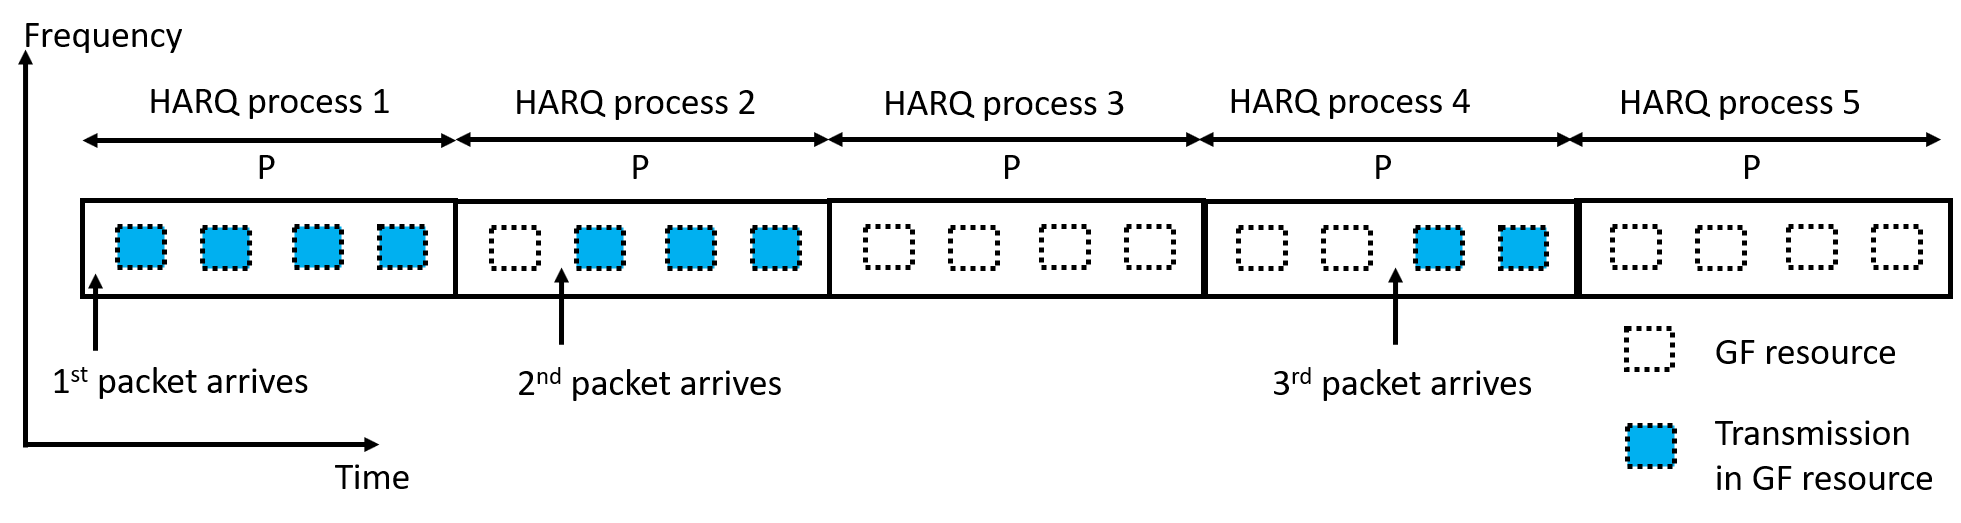
\includegraphics[scale=0.27]{fig16.png}}
\caption{Less than K repetitions in CG UL transmission.}
\label{fig16}
\end{figure}

It is evident that when the packet comes after the first CG occasions in a period, the UE transmits the packet with a smaller number than the number configured by repK. It degrades the reliability of UL transmission. The situation becomes more severe for the URLLC UEs with high reliability requirement. Moreover, latency of a transmission also increases because with a smaller number of repetitions, the gNB has a higher probability of failing to decode the packet and needs to schedule a retransmission. In that case, the UE needs to wait the gNB to decode the repetitions of the packet and transmit an UL grant to reschedule a retransmission if necessary and it has a huge impact on latency.

\section{Reserved resources to ensure the number of repetitions} \label{32}
\subsection{Reserved resources}
To make the URLLC UEs achieve the strict requirements, a strategy to ensure that the UEs can transmit the number of repetitions as configured by repK from higher layer is indispensable. Reserved periodic resources are proposed to be created and assigned to multiple UEs by the gNB so that they are likely to retransmit data in case the transmissions in the reserved resources are necessary to ensure the configured number of repetitions. These reserved resources have the same periodicity as the CG resources.

\begin{figure}[htbp]
\centerline{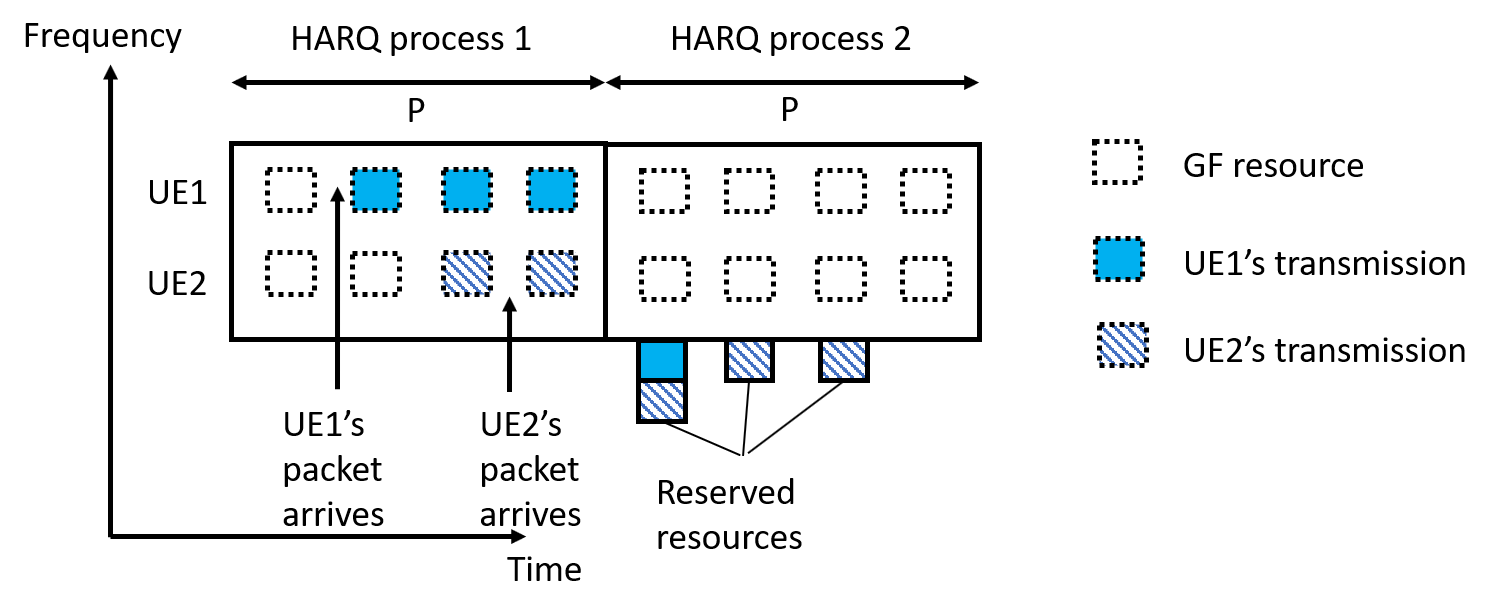
\includegraphics[scale=0.30]{fig17.png}}
\caption{Reserved resources for repetitions.}
\label{fig17}
\end{figure}

The use of reserved resources is shown in Fig.~\ref{fig17}. There are 2 UEs considered with CG resources in different bandwidth and each UE is configured with repK = 4. UE1's data comes after the first CG occasion in the first period so it only can do 3 repetitions in the period. In order to attain 4 repetitions, the UE1 retransmits data in the first reserved resource of the next period. Similarly, UE2's data arrives at the last CG occasion and only one repetition can be made. Thus, the UE2 uses the 3 reserved resources in the next period to achieve the configured number of repetitions.

\subsection{System model}\label{322}

\begin{figure}[htbp]
\centerline{
\includegraphics[scale=0.3]{fig18.png}}
\caption{UL transmission resources' distribution.}
\label{fig18}
\end{figure}

The system in Fig.~\ref{fig18} considered to calculate collision probability in the reserved resources contains $N$ UEs. These $N$ UEs are configured by the gNB to transmit in the periodical CG resources with the number of repetitions $K$ set by parameter repK. The UEs transmit the automatic repetitions of a packet in the consecutive CG resources. The CG resources in one frequency band can be shared among the UEs in a group. A period $P$ corresponding to a HARQ process consists of CG transmission occasions equal to the number of repetitions $K$. The results derived below are also valid if the number of CG transmission occasions in a period are bigger than $K$. The reserved resources ($K-1$ reserved resources) are configured periodically as CG resources in each period $P$. These resources are shared among the $N$ UEs to retransmit data in case the number of repetitions that they can carry out in one period are less than the configured one. Each reserved resource has size of $M_{i}$ blocks with index $i$ indicating that the reserved resource is at the $i$th transmission occasion of a period. The size of each block in the reserved resources is the same as that of the CG resource in one transmission occasion.

The arrival of data for each UE follows a Poisson process with the average number of random access events in an interval $\lambda$ calculated from the period between the CG resources $T$ and an average packet inter-arrival time $\mu$: $\lambda$ = $T/\mu$.

\subsection{Optimization of reserved resource size}

With random access, the $N$ UEs in system are allowed to use any block in the reserved resources of a specific transmission occasion if they need to do the transmissions in order to fulfill the configured number of repetitions.

A general equation of collision probability for the reserved resource at any transmission occasion in a period can be derived as \useshortskip

\begin{equation}
P_{ci} = 1 - (\frac{M_{i}-1+e^{-\lambda(K-i)}}{M_{i}})^{N-1},\label{eq7}
\end{equation}
where
$i \in [1, K-1]$ is index indicating the position of the reserved resource based on the position of transmission occasion in a period.

From \eqref{eq7} with a set of parameters  $\lambda, N, K, i,$ and $P_{ci}$, the size of the reserved resources at any transmission occasion can be calculated. To guarantee the reliability of transmission in the reserved resources in comparison to that in the CG resources, the target probability $P_{ci}$ is chosen to be approximate to $P_{c\_CG}$. If $P_{ci}$ is set to have the same value in all the reserved resources, the trend of reserved resources' size in terms of their positions in a period is: $M_1 > M_2 > M_3 > ... > M_{K-1}$. The size of the reserved resources to achieve a target probability decreases gradually from the first to the last reserved resource in a period. The design of the reserved resources following this decreasing trend instead of using the same size for all of the reserved resource brings an efficiency of resource consumption because the size is optimized particularly for each reserved resource.

\subsection{Group access to the reserved resources}

In group access approach, one UE is only allowed to access and uses a specific part of the reserved resource pre-configured by the gNB. One part of the reserved resource is assigned and shared among a group of the UEs.

For a group of the UEs accessing to a part of the reserved resources, the collision probability is calculated by \eqref{eq7} as random access approach. The size of the whole reserved resource in each transmission occasion is sum of all parts assigned to the UE groups to guarantee a target probability. 

Group access approach reduces the decoding burden in the gNB. To decode a retransmitted packet, the gNB only needs to search a part of the reserved resource instead of the entire reserved resource as random access approach. Thereby, power consumption and processing time drop dramatically. 

\subsection{Numerical results}\label{324}

From \eqref{eq7}, the number of the UEs that the system can support can be found. Besides, the number of resource blocks in each reserved resource are also calculated to sustain that system.

The simulation starts with the reserved resource in the first transmission occasion of a period. The set of parameters is $M_1=10, K=4, \lambda=1.25\times10^{-4}$.

Fig.~\ref{fig19}\subref{19a} shows collision probability in the reserved resource in the first transmission occasion in terms of the number of the UEs sharing that resource. From the graph, we see that if the target collision probability ($P_{c1}$) is 10\textsuperscript{-3}, the system can support 28 UEs in the first reserved resources.

\begin{figure}[htbp]
\centering
\subfloat[Collision probability with respect to the number of the UEs.\label{19a}]{%
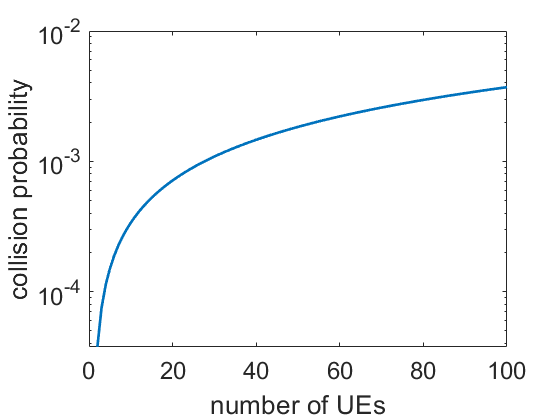
\includegraphics[scale=0.35]{fig19.png}}
\hspace{2em}
\qquad
\subfloat[Collision probability of the second reserved resource.\label{19b}]{%
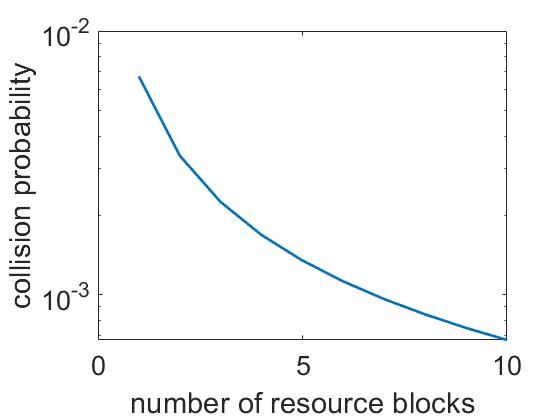
\includegraphics[scale=0.35]{fig20.png}}
\hspace{2em}
\caption{Collision probability.}
\label{fig19}
\end{figure}

As mentioned in Section \ref{322}, the CG resources in a frequency band can be shared by a group of the UEs. 28 UEs calculated above can be divided in to 4 groups with 7 UEs in each group. The collision probability in the CG resources is $7.5\times10^{-4}$ that is approximate to the collision probability of 10\textsuperscript{-3} in the reserved resource.

When all the parameters ($\lambda, N, K$ and $P_{ci}$) are kept the same, the sizes of the reserved resources in the second and the third transmission occasions are calculated as shown in Table~\ref{tab6}.
%KHOA BEGIN
% THem ti khoang trong' duoi table, chon medskip, bigskip hoac smallskip
%\smallskip
%\smallskip
%\bigskip
\begin{table}[htbp]
\caption{Sizes of the reserved resources with $K=4$ and random access}
\begin{center}
\begin{tabular}{|p{10em}|p{2em}|p{2em}|p{2em}|}
 \hline
 \textbf{\textit{Position of reserved resources}} & $1$ &$2$ &$3$ \\ 
 \hline
 \textbf{\textit{Number of blocks}} & $10$ &$7$ &$3$ \\

%  increase row height, number of & = number of collumn
% &&&&&\\[-1em]
 
 \hline
\end{tabular}
\label{tab6}
\end{center}
\end{table}

%\medskip
%KHOA END

The percentage of resources saved in comparison to using the same size of 10 resource blocks for all the resources is: $(1 - (10+7+3)/(10\times3))\times100\% = 33\%$.

Fig.~\ref{fig19}\subref{19b} illustrates collision probability with respect to the reserved resource's size in the second transmission occasion.

Another scenario is considered with a bigger number of repetitions: $M_1=10, K=8, \lambda=1.25\times10^{-4}$ .

The system can support 12 UEs in the first reserved resources to achieve Pc target of 10\textsuperscript{-3}. These UEs can be divided into 2 groups with 6 UEs in one group that each group uses the CG resources in one bandwidth part. The collision probability in CG regions of a group of 6 UEs as scheduled above is: $6.25\times10^{-4}$.
With 12 UEs, the sizes of the reserved resources in the transmission occasions are shown in Table~\ref{tab7}.

\begin{table}[htbp]
\caption{Sizes of the reserved resources with $K=8$ and random access}
\begin{center}
\begin{tabular}{|p{5em}|p{2em}|p{2em}|p{2em}|p{2em}|p{2em}|p{2em}|p{2em}|}
 \hline
 \textbf{\textit{Position of reserved resources}} & $1$ &$2$ &$3$ & $4$ &$5$ &$6$ &$7$\\ 
 \hline
 \textbf{\textit{Number of blocks}} & $10$ &$8$ &$7$ & $6$ &$4$ &$3$ &$2$\\

%  increase row height, number of & = number of collumn
% &&&&&\\[-1em]
 
 \hline
\end{tabular}
\label{tab7}
\end{center}
\end{table}

The percentage of resources saved in comparison to using the same size of 10 resource blocks for all the resources is: $(1 - (10+8+7+6+4+3+2)/(10\times7)) \times100\% = 42.86\%$

As can be seen from two scenarios, the use of reserved resources with optimization from \eqref{eq7} brings an efficiency of resource utilization, especially for high configured number of repetitions. The resources needed are less than the approach of choosing blindly the same sizes for all reserved resources in different transmission occasions while still guarantees the number of repetitions with a target reliability.

Moreover, in the conventional scheme in 3GPP Release 15, the UE needs to wait until the next period if it cannot do the configured number of repetitions in the current period to fulfill the reliability requirement. Therefore, with $K=4$ and 4 transmission occasions in a period, in the worst case, the UE must wait 3 transmission occasions equal to 3 slots or 0.75ms with SCS 60kHz. This latency is close to the URLLC requirement of 1ms and causes the UEs not be able to make 4 repetitions as configured in the next period. In comparison, the proposed scheme allows the UE to start the transmission immediately and reach the configured number of repetitions in target latency of 1ms (4 repetitions consume 1ms with SCS 60kHz) as well as meet the reliability requirement.

The proposals related to reserved resources for UL transmission with less than K repetitions is published in EuCNC 2019 paper "Optimal reserved resources to ensure the repetitions in Ultra-Reliable Low-Latency Communication Uplink Grant-free transmission" \cite{b9}. 

\section{Explicit feedback structure and scheduling request to improve UE detection}\label{33}

\subsection{Operation of explicit HARQ feedback structure}\label{331}

The HARQ structure in UL CG transmission is timer-based. This means that there is no explicit acknowledgement (ACK) feedback sent from the gNB to the UE if data is decoded correctly. Instead, the UE uses a timer. If it does not receive an UL grant to schedule a retransmission at the end of time configured in the timer, the transmission is considered as successful. This structure has a drawback because the UE cannot differentiate between a successful transmission and a miss-detection when the gNB cannot decode DMRS to identify the UE and transmits UL grant. Therefore, in case of miss-detection, the UE does not receive any signal from the gNB, it assumes a successful transmission and drops data in buffer. This behavior impacts reliability of a transmission and becomes more severe in less-than-K-repetitions situation. Once the UE is not able to carry the configured number of repetitions, the QoS of transmission is badly affected and there is a higher probability that the gNB cannot decode DMRS sequence. It leads to a degradation of URLLC transmission due to packet dropped by the UE. To handle the issue with CG transmissions with less than K repetitions, we propose to use explicit HARQ feedback from the gNB. 

In the proposed technique, whenever the UE transmits less than K repetitions, the TB in question is supposed to operate with explicit HARQ based feedback. In general, the gNB can identify transmissions with less than K repetitions thanks to DMRS detection and CG window boundary knowledge. When the gNB fails to identify the transmitting UE and sends no ACK or UL grant to this UE, the UE upon expiry of configured HARQ timer re-transmits automatically the TB. 

\subsection{Improving reliability-latency by flexibly transmitting an additional Scheduling Request} \label{332}

In this section, another scheme is proposed to deal with the problem of less-than-K repetitions. In this scheme to improve the reliability of UL CG transmissions, whenever the UE transmits less than the configured number of repetitions for a TB, it sends SR to the gNB, in parallel to transmission of TB with less than K repetitions. This SR provides a sort of diversity mechanism in parallel to the transmission of the TB.

Release 15 does not allow transmission of Physical uplink control channel (PUCCH) and Physical uplink shared channel (PUSCH) simultaneously. The UE transmits UCI encoding SR, HARQ feedback, etc on PUCCH. Therefore, the UE multiplexes UCI and PUSCH if it wants to transmit uplink control information (UCI) while sending PUSCH. This strategy allows the UE to transmit SR in case of less than K repetitions. However, in UCI and PUSCH  multiplexing, if the gNB cannot detect DMRS of PUSCH due to bad channel, there is high probability that the gNB also cannot decode UCI (SR) to find the UE ID. Thus, multiplexing strategy might not enhance the performance of UE ID detection. For this reason, SR should be configured to be transmitted on the configured PUCCH resources. The gNB upon receiving PUCCH and PUSCH from the same UE will understand that the SR in PUCCH is for the same TB sent in PUSCH for the UE that is only able to make less than K repetitions.

\subsection{Numerical results and performance evaluation}

\begin{table}[htbp]
\caption{Simulation parameters}
\begin{center}
\begin{tabular}{|p{8em}|p{8em}|}
 \hline
 \textbf{Parameters} & \textbf{Values}\\
 \hline
 Waveform & CP-OFDM\\
 \hline
 Subcarrier spacing & 60kHz\\
 \hline
 Channel model & Rician\\
 \hline
 K factor & 1\\
 \hline
 Number of allocated PRB & 8\\
 \hline
 DMRS detection mechanism & Time-domain correlation\\
 

%  increase row height, number of & = number of collumn
% &&&&&\\[-1em]
 
 \hline
\end{tabular}
\label{tab11}
\end{center}

\end{table}

\begin{figure}[htbp]
\centerline{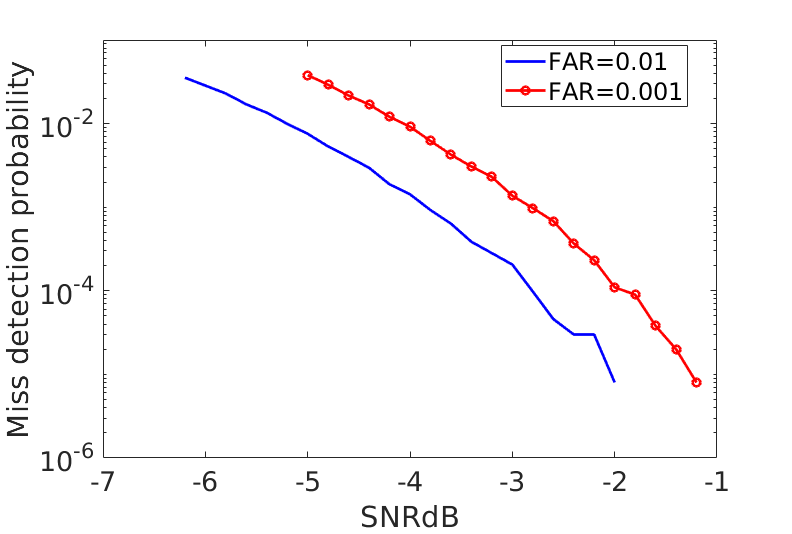
\includegraphics[scale=0.3]{fig26.png}}
\caption{DMRS detection performance.}
\label{fig26}

\end{figure}

Simulation parameters for the performance of DMRS detection of each repetition in Fig.~\ref{fig26} are shown in Table~\ref{tab11}. For each DMRS detection, the correlation result is compared with a threshold to determine whether DMRS exists or not. This threshold is chosen according to a target false alarm rate (FAR) indicating the cases that the gNB determines the existence of DMRS while in reality there is no DMRS transmitted. A higher threshold is required for a lower FAR but also results in more missed detection. As DMRS dectection is mandatory for channel estimation to decode data as well as for recognizing UE ID to reschedule a retransmission if necessary in conventional scheme, a degradation of DMRS detection due to a smaller number of repetitions than configured makes the system not be able to support reliability URLLC requirement.

\begin{table}[htbp]
\caption{Performance comparison of different schemes when data comes after the first occasion in a period at $SNR = -5dB$ and $FAR = 0.001$}
\begin{center}
\begin{tabular}{|p{6em}|p{4em}|p{4em}|p{4em}|p{4em}|p{4em}|}
 \hline
 \textbf{Case} & \textbf{Starting time offset (ms)}&\textbf{Number of repetitions}&\textbf{UE ID miss-detection probability}&\textbf{Retrans in ID miss-detection}&\textbf{Total UE ID miss-detection probability}\\
 \hline
 Conventional transmission&$0$&$3$&$5.5\times10\textsuperscript{-5}$&$0$&$5.5\times10\textsuperscript{-5}$\\
 \hline
 Conventional transmission with the UE waiting the next period&$0.75$&$1$&$0.038$&$0$&$0.038$\\
 \hline
Transmission with explicit ACK&$0$&$3$&$5.5\times10\textsuperscript{-5}$&$1$&$2.1\times10\textsuperscript{-6}$\\
\hline
Transmission with SR&$0$&$3$&$2.1\times10\textsuperscript{-6}$&$0$&$2.1\times10\textsuperscript{-6}$\\
 \hline
\end{tabular}
\label{tab12}
\end{center}
\end{table}

\begin{table}[htbp]
\caption{Performance comparison of different schemes when data comes after the second occasion in a period at $SNR = -5dB$ and $FAR = 0.001$}
\begin{center}
\begin{tabular}{|p{6em}|p{4em}|p{4em}|p{4em}|p{4em}|p{4em}|}
 \hline
 \textbf{Case} & \textbf{Starting time offset (ms)}&\textbf{Number of repetitions}&\textbf{UE ID miss-detection probability}&\textbf{Retrans in ID miss-detection}&\textbf{Total UE ID miss-detection probability}\\
 \hline
 Conventional transmission&$0$&$2$&$10\textsuperscript{-3}$&$0$&$10\textsuperscript{-3}$\\
 \hline
 Conventional transmission with the UE waiting the next period&$0.5$&$2$&$10\textsuperscript{-3}$&$0$&$10\textsuperscript{-3}$\\
 \hline
Transmission with explicit ACK&$0$&$2$&$10\textsuperscript{-3}$&$2$&$2.1\times10\textsuperscript{-6}$\\
\hline
Transmission with SR&$0$&$2$&$5.5\times10\textsuperscript{-5}$&$0$&$5.5\times10\textsuperscript{-5}$\\
 \hline
\end{tabular}
\label{tab13}
\end{center}
\end{table}

\begin{table}[htbp]
\caption{Performance comparison of different schemes when data comes after the third occasion in a period at $SNR = -5dB$ and $FAR = 0.001$}
\begin{center}
\begin{tabular}{|p{6em}|p{4em}|p{4em}|p{4em}|p{4em}|p{4em}|}
 \hline
 \textbf{Case} & \textbf{Starting time offset (ms)}&\textbf{Number of repetitions}&\textbf{UE ID miss-detection probability}&\textbf{Retrans in ID miss-detection}&\textbf{Total UE ID miss-detection probability}\\
 \hline
 Conventional transmission&$0$&$1$&$0.038$&$0$&$0.038$\\
 \hline
  Conventional transmission with the UE waiting the next period&$0.25$&$3$&$5.5\times10\textsuperscript{-5}$&$0$&$5.5\times10\textsuperscript{-5}$\\
 \hline
Transmission with explicit ACK&$0$&$1$&$0.038$&$3$&$2.1\times10\textsuperscript{-6}$\\
\hline
Transmission with SR&$0$&$1$&$10\textsuperscript{-3}$&$0$&$10\textsuperscript{-3}$\\
 \hline
\end{tabular}
\label{tab14}
\end{center}
\end{table}

In considered system, periodicity $P$ of HARQ process is 4 slots spreading in 1ms with SCS of 60kHz. The UE is configured to transmit 4 repetitions. As specified in \cite{ad6}, each slot only contains one repetition so one repetition consumes 0.25ms and the UE needs 4 slots to carry out all 4 configured repetitions and satisfies URLLC latency budget of 1ms.

Table~\ref{tab12}, Table~\ref{tab13} and Table~\ref{tab14} show the performance of DMRS detection at SNR of -5dB and FAR of 0.001 in various schemes and arrival time of data. As can be seen with conventional  transmission, due to the constraint of boundary of a period $P$, the UE cannot transmit 4 configured repetitions and it affects DMRS detection's performance. The later the packet comes, the worse DMRS detection is. In the timer-based feedback of the conventional scheme, the packet is lost because the UE assumes a successful transmission in case of DMRS miss-dection. Even if the UE waits for the next period with the intention of carrying of K repetitions configured as the second scheme, it also cannot achieve that intention because of URLLC latency requirement of 1ms. The more time the UE waits, the less time it has to transmit the repetitions. In consequence, it also cannot transmit K repetitions and DMRS miss-detection grows.

The presence of explicit feedback solves the problem of an increase of DMRS-miss detection because it helps the UE differentiate between a successful transmission and DMRS-miss detection. Therefore, the UE is able to retransmit packet even if the gNB does not detect UE ID by DMRS detection and reliability is guaranteed (total miss-detection probability of $2.1\times10\textsuperscript{-6}$ smaller than the conventional schemes) as shown in Table~\ref{tab12}, Table~\ref{tab13} and Table~\ref{tab14}.

These three tables also show that an additional SR transmitted in parallel with data provides another chance for the gNB to identify the UE and compensates for the missing repetitions due to boundary constraint so system performance is enhanced. 

The proposals related to two-step strategy is published in ISWCS 2019 paper "Strategies to meet the configured repetitions in URLLC Uplink Grant-Free transmission" \cite{ad100}. 

\chapter{Future works} \label{S4}

The works in the first year focused on UL CG transmission in FDD. The works in the second year are being expanded to the existing problems of CG transmission in TDD. The application of CG transmission in DL to increase reliability and reduce latency are also being considered. These researches are following the progress of 3GPP meetings and the feature in the next releases ( the upcoming release is in December 2019).

\section{Repetition across period boundary in TDD}

\begin{figure}[htbp]
\centerline{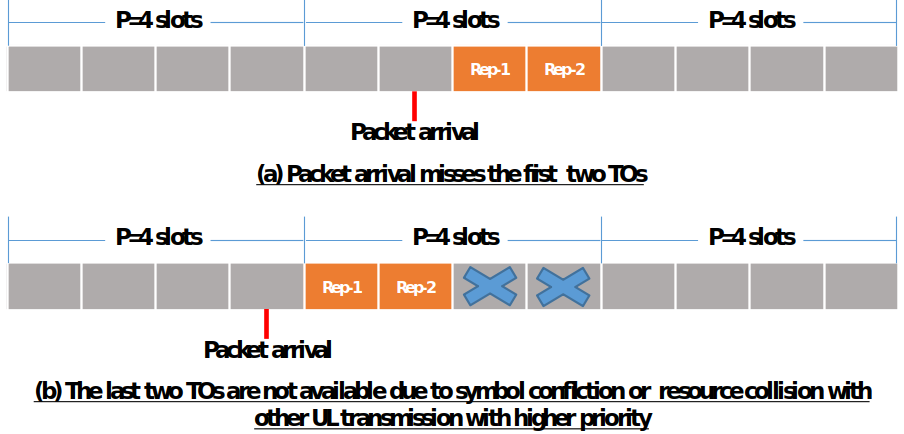
\includegraphics[scale=0.35]{fig30.png}}
\caption{The two cases that cause less-than-K-repetition transmission.}
\label{fig30}
\end{figure}

In Fig.~\ref{fig30}a, the UE cannot transmit 4 repetitions as configured du the late arrival of a packet. This scenario has been discussed in Chapter \ref{S3}. There is another scenario that causes a smaller number of repetitions transmitted than configuration that is shown in Fig.~\ref{fig30}b. A packet arrives before the beginning of a HARQ period,  but the UE also cannot transmit all 4 repetitions. The reason is that this period contains two DL slotss. In TDD, the UE is not allowed to transmit data in these slots. Another reason that can explain this situation is the appearance of another UL transmission with a higher priority in the last two slots. Both two reasons cause a transmission with less repetitions than configuration that reduce reliability of URLLC transmission.

\begin{figure}[htbp]
\centerline{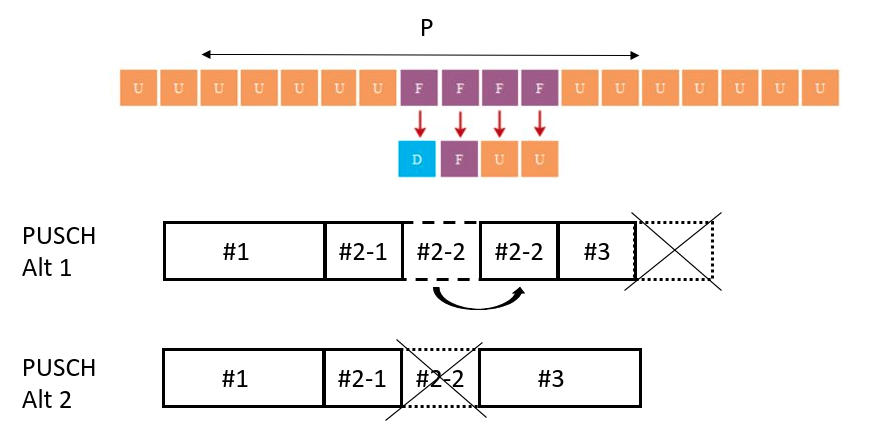
\includegraphics[scale=0.35]{fig31.png}}
\caption{Less-than-K-back-to-back-repetition transmission in TDD .}
\label{fig31}
\end{figure}

In Release 16, 3GPP supports back-to-back repetitions of a packet in mini-slot as shown in Fig.~\ref{fig31} instead of one repetition in each slot as in Fig.~\ref{fig30}. In this technique, the problem of less-than-K transmission due to UL/DL symbol conflict still exists. The UE has two options to proceed the repetitions. In the first option as shown in Fig.~\ref{fig31}, the UE segments the second repetition in two part and postpones the second segment until the next available UL symbol after the DL and flexible symbols. However, due to the delay, the UE cannot transmit the entire third repetition because of period boundary. In the second option, the UE also do segmentation at UL/DL symbol transition but drops the second segment. Both two options cause a degradation of reliability.

The problem of CG transmission in TDD requires a technique in physical layer design to guarantee URLLC requirements. The techniques published in the papers can be considered as a candidate to solve this problem. Certainly, these techniques are not be able to be applied directly in the system. They require the modification to be suitable to TDD configuration.

One solution is to use an UCI transmitted in parallel with data to inform the gNB about the UE ID. Thanks to this known UE ID, the gNB knows where to send UL grant for a retransmission if necessary. There is no confusion in the UE ID if there are the repetitions in different HARQ periods so the UE is allowed to transmit across the period boundary to achieve the configured number of repetitions.

A second solution under research is to use reserved resources after the DL or flexible symbols. The reserved resource is used by the UE to transmit the repetitions dropped due to UL/DL symbol conflict. This method required a certain gap between the DL symbols and the next UL symbols used for the repetitions. If there is no gap, the UE might transmit two repetitions simultaneously: one repetition in the CG resources as configure and one repetition in the reserved resource. Due the limitation of power at the UE, a parallel transmission make the power level in each transmission decrease and the target to achieve a better reliability with the reserved resource is not fulfilled.

\section{ DL SPS transmission}

In Release 15, the DL SPS resources can be configured by the gNB to use to transmit physical downlink shared channel (PDSCH). DL SPS resources is similar to UL CG resources. The gNB transmits PDSCH without transmitting physical downlink control channel (PDCCH) to indicate transmission parameters as usual. The use of DL SPS resources reduces latency due to PDCCH blocking, transmission and processing time of PDCCH. It also increases reliability when the probability of PDCCH error is eliminated. In the normal DL transmission, if the UE cannot decode PDCCH, it also cannot decode PDSCH because the location of PDSCH is unknown. 

However, the periodicity of DL SPS resources is much higher than URLLC requirement of 1 ms. In Release 15, the minimum periodicity is 10 ms. Thus, it is not suitable to use DL SPS resources in URLLC transmission.

Nevertheless, in recent meetings, 3GPP agreed to support DL SPS resources with periodicity of a slot. The shortest periodicity is 0.5 ms equivalent to 1 slot with SCS of 30 kHz. This agreement makes the use of DL SPS resources for URLLC DL transmission feasible. 

One scheme under research is to use the DL SPS resources for the retransmission. Due to the strict latency, the retransmission with both PDCCH and PDSCH is not possible in almost the scenarios with different SCS and the period of sub-slot. Thus, in the researched scheme, the gNB starts the initial transmission with PDCCH and PDSCH as conventional scheme. Subsequently, if it does not receive feedback because of PDCCH failure at the UE or NACK feedback because of PDSCH failure at the UE, it quickly sends the second PDSCH in the DLC SPS resources to save the preparing time,transmission time and decoding time of PDCCH. This scheme increase reliability and reduce resource consumption because the reliability of the first PDCCH and PDSCH can be relaxed, the UE still has another chance to decode correctly the packet with the second potential transmission.

\section{Other works}

The final target of the thesis is to make URLLC design achieve the strict requirements in different scenarios of the applications. The works in future are to continue to locate the problems in URLLC design that prevent the system from attaining high reliability and low latency. The aspects of energy and resource consumption are going to be taken into account in the design process. The problems identified and the solutions proposed will be aligned with the progress of the discussions in 3GPP meetings. 

The features of URLLC design are also being researched to be cooperated in the design of V2X and transmission NR unlicensed spectrum.

\chapter{Conclusion} \label{S5}

\section{The results of the works}
URLLC requires strict reliability and latency requirements but there are still problems in physical layer design that make the system unable to achieve those requirements. The techniques proposed in this paper helps the URLLC transmissions overcome two major problems: first is the successfull eMBB and URLLC multiplexing, the second is to ensure QoS targets when URLLC UEs can not transmit less than K repetitions with CG transmissions. 

In the problem of multiplexing between eMBB and URLLC UEs, a mechanism using PI avoids the collision between the GB eMBB and URLLC UEs. This mechanism chooses the eMBB candidates for cancellation and informs these UEs by 1-bit flag embedded in UL grant. The UEs that receive an active flag increase monitoring periodicity and capability. Besides that, an overlap indication with explicit feedback or additional SR are used to enhance the performance of CG URLLC multiplexing with GB eMBB. The simulation shows that these techniques reduce URLLC packet loss due to DMRS miss-detection in the transmission suffering from the interference from the eMBB UEs. 

For the problem of less than the configured number of repetitions, three techniques, the optimal reserved resources, explicit feedback and additional SR, are proposed over the prior art. The advantages and disadvantages of each method have been shown by the calculation and simulations. 

\section{Achievements}
\begin{itemize}
    \item  Trung-Kien Le, Umer Salim, Florian Kaltenberger, ``Optimal reserved resources to ensure the repetitions in Ultra-Reliable Low-Latency Communication Uplink Grant-free transmission'',  2019 European Conference on Networks and Communications (EuCNC), June 2019.
    \item Trung-Kien Le, Umer Salim, Florian Kaltenberger, ``Strategies to meet the configured repetitions in URLLC Uplink Grant-Free transmission'',  2019 16th International Symposium on Wireless Communication Systems (ISWCS), August 2019.
    \item Trung-Kien Le, Umer Salim, Florian Kaltenberger, ``Improving Ultra-Reliable Low-Latency Communication in multiplexing with Enhanced Mobile Broadband in grant-free resources'', 2019 IEEE International Symposium on Personal, Indoor and Mobile Radio Communications (PIMRC), September 2019.
    \item Trung-Kien Le, Umer Salim, Florian Kaltenberger, ``Control and data channel combining in Ultra-Reliable Low-Latency Communication'', Asilomar Conference on Signals, Systems, and Computers, November 2019.
\end{itemize}

\section{Plan Individuel de Formation Doctorale}
I completed the following courses:
\begin{itemize}
    \item Mobile communication systems (42 hours)
    \item French course 1 (20 hours)
    \item French course 2 (20 hours)
\end{itemize}


\clearpage

\begin{thebibliography}{9}
\bibitem{ad1} 3GPP TR 38.913 v15.0.0, ``Study on scenarios and requirements for next generation access technologies.''
\bibitem{ad2} Huawei, HiSilicon, Nokia, Nokia Shanghai Bell, ``New SID on Physical Layer Enhancements for NR URLLC''. 3GPP RP-182089, TSG-RAN\#81, Gold Coast, Australia, Sept 10--13, 2018.
\bibitem{ad3} 3GPP TS 38.214 v15.3.0, ``Physical layer procedures for data.''
\bibitem{ad4} Huawei, HiSilicon, ``UL inter-UE transmission prioritization and multiplexing'', 3GPP R1-1810158, RAN1\#94bis, Spokane, Chengdu, China, 8--12 October, 2018.
\bibitem{ad5} ZTE, ``UL inter-UE multiplexing between eMBB and URLLC'', 3GPP R1-1900074, RAN1 AH 1901, Taipei,  21--25 January, 2019.
\bibitem{ad6} 3GPP TS 38.211 v15.3.0, ``Physical channels and modulation.''
\bibitem{ad7} 3GPP TR 38.802 v14.2.0, ``Study on new radio access technology physical layer aspects.''
\bibitem{ad8} Huawei, HiSilicon, ``UL inter-UE transmission prioritization and multiplexing'', 3GPP R1-1810158, RAN1\#94bis, Spokane, Chengdu, China, 8--12 October, 2018.
\bibitem{ad9} ZTE, ``UL inter-UE multiplexing between eMBB and URLLC'', 3GPP R1-1900074, RAN1 AH 1901, Taipei,  21--25 January, 2019.
%\bibitem{b4} Sony, ``On Enhancement of UL grant-free transmissions'', 3GPP R1-1808345, RAN1\#94, Gothenburg, Sweden, August 20--24, 2018.
\bibitem{ad10}  Sony, ``Inter-UE uplink multiplexing of URLLC \& eMBB traffics'', 3GPP R1-1812745, RAN1\#95, Spokane, USA, November 12--16, 2018.
\bibitem{ad11}  Institute for Information Industry (III), ``UL Inter UE Tx prioritization/multiplexing'', 3GPP R1-1813481, RAN1\#95, Spokane, USA, November 12--16, 2018.
\bibitem{ad12}  NEC, ``UL inter-UE multiplexing of eMBB and URLLC'', 3GPP R1-1812419, RAN1\#95, Spokane, USA, November 12--16, 2018.
\bibitem{ad13}  C.-P. Li, J. Jiang, W. Chen, T. Ji, and J. Smee, ``5G ultra-reliable and low-latency systems design,'' in 2017 European Conference on Networks and Communications (EuCNC), Jun. 2017, pp. 1-5. 
\bibitem{ad14} D. Tse and P. Viswanath, Fundamentals of Wireless Communication. Cambridge University Press, 2005. 
\bibitem{ad15} 3GPP TS 38.212 v15.3.0, ``Multiplexing and channel coding.''
\bibitem{ad16} 3GPP TS 38.331 v15.3.0, ``Radio Resource Control (RRC) protocol specification.''
\bibitem{ad17} Ericsson, ``Enhancement of Configured Grant for NR URLLC'', 3GPP R1-1812162, RAN1\#95, Spokane, USA, November 12--16, 2018.
\bibitem{ad18} Huawei, HiSilicon, ``Enhanced UL configured grant transmissions'', 3GPP R1-1812226, RAN1\#95, Spokane, USA, November 12--16, 2018.
\bibitem{ad19} Intel Corporation, ``On enhanced Configured Grant PUSCH for eURLLC'', 3GPP R1-1812506, RAN1\#95, Spokane, USA, November 12--16, 2018.
\bibitem{ad20} Sony, ``Discussion on enhanced UL grant-free transmissions'', 3GPP R1-1812746, RAN1\#95, Spokane, USA, November 12--16, 2018.
\bibitem{ad23} Chairman's notes RAN1 \#96bis, Xi'an, China, April 8--12,2019.
\bibitem{ad24} Chairman's notes RAN1 \#97, Reno, USA, May 13--17,2019.
\bibitem{ad21} R. breu, G. Berardinelli, T. Jacobsen, K. Pedersen and P. Mogensen, ``A Blind Retransmission Scheme for Ultra-Reliable and Low Latency Communications'', 2018 IEEE 87th Vehicular Technology Conference (VTC Spring), June 2018.
\bibitem{ad22} Z. Zhou, R. Ratasuk, N. Mangalvedhe and A. Ghosh, ``Resource Allocation for Uplink Grant-Free Ultra-Reliable and Low Latency Communications'', 2018 IEEE 87th Vehicular Technology Conference (VTC Spring), June 2018.
\bibitem{b9} Trung-Kien Le, Umer Salim, Florian Kaltenberger, ``Optimal reserved resources to ensure the repetitions in Ultra-Reliable Low-Latency Communication Uplink Grant-free transmission'',  2019 European Conference on Networks and Communications (EuCNC), June 2019.
\bibitem{ad100} Trung-Kien Le, Umer Salim, Florian Kaltenberger, ``Strategies to meet the configured repetitions in URLLC Uplink Grant-Free transmission'',  2019 16th International Symposium on Wireless Communication Systems (ISWCS), August 2019.
\bibitem{ad99} Trung-Kien Le, Umer Salim, Florian Kaltenberger, ``Improving Ultra-Reliable Low-Latency Communication in multiplexing with Enhanced Mobile Broadband in grant-free resources'', 2019 IEEE International Symposium on Personal, Indoor and Mobile Radio Communications (PIMRC), September 2019.
\bibitem{ad101} Trung-Kien Le, Umer Salim, Florian Kaltenberger, ``Control and data channel combining in Ultra-Reliable Low-Latency Communication'', Asilomar Conference on Signals, Systems, and Computers, November 2019.
\end{thebibliography}
\addcontentsline{toc}{chapter}{References}
\clearpage


\begin{comment}


\appendix
\addcontentsline{toc}{chapter}{Appendix}
\renewcommand{\thesection}{\Alph{section}}
\section{Supporting mechanism of preemption indication in eMBB and URLLC multiplexing}\label{Ap1}
\subsection{UL Pre-Emption Indication for eMBB UE}
\subsubsection{Basic scheme}

Some scheme using PI has been discussed in 3GPP tdocs to multiplex eMBB and URLLC in different scenarios.

\textbf{\underline{Multiplexing between eMBB and URLLC grant-based (GB) transmission}}
\begin{figure}[htbp]
\centerline{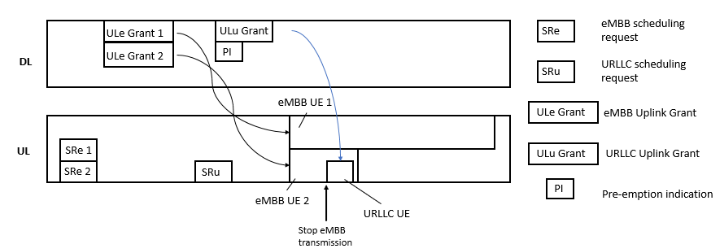
\includegraphics[scale=0.35]{fig2.png}}
\caption{Multiplexing between eMBB GB and URLLC GB transmission.}
\label{fig2}
\end{figure}

When the eMBB UEs have data to transmit, they send SR and receive UL grant from the gNB with resource allocation. After resources are allocated to the eMBB UEs, an URLLC UE also has data to transmit and request resources from the gNB as shown in Fig.~\ref{fig2}. Due to latency requirement of URLLC, the gNB may have to allocate the URLLC UE to resources scheduled to the eMBB UEs. To avoid an interference among the UEs with different requirements, the gNB sends PI to the eMBBs in order to cancel or stop temporarily the eMBB transmission.

\textbf{\underline{Multiplexing between eMBB grant-based (GB) and URLLC configured grant (CG) transmission}}

\begin{figure}[htbp]
\centerline{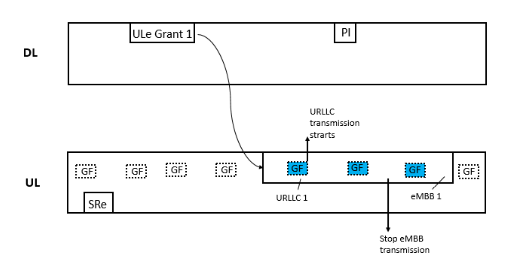
\includegraphics[scale=0.35]{fig3.png}}
\caption{Multiplexing between eMBB GB and URLLC CG transmission.}
\label{fig3}
\end{figure}

In the uplink, there are CG regions where the URLLC UEs transmit without explicit SR. To attain a better resource utilization, the gNB can schedule the eMBB UE to transmit in the CG region dedicated to the URLLC UE because the arriving rate of URLLC data might be low. When the gNB allocates resources for the eMBB UEs on both grant-based (GB) and configured grant (CG) region, CG URLLC transmission may collide with eMBB transmission because the gNB does not know URLLC transmission in advance by SR.

If the URLLC UE transmits data in the configured regions that are overlapped with the eMBB UE, the gNB detects the transmission and perceives that it is carried out over the CG regions scheduled to the eMBB UE due to DMRS sequences. Consequently, the gNB sends PI to the eMBB UE to cancel or stop immediately their transmissions. Therefore, the URLLC UE has the collision-free CG to do retransmission in order to achieve the requirement of reliability. As in Fig.~\ref{fig3}, the URLLC UE has one collision-free CG for retransmission after the eMBB transmission is stopped.

URLLC transmission is mini-slot transmission. Thereby, in case PI is transmitted to the eMBB UEs, it must be done in mini-slot level to be likely to stop the transmission in time and satisfy the traffic critical delay. This design requires that the eMBB UEs monitor PI in mini-slot level. However, the eMBB UEs transmit data in slot level and also only monitors DCI in slot level. This means that if DCI is used as PI, the eMMB UEs are required to increase monitoring periodicity. Monitoring capability of the eMBB UEs also must be enhanced with a growth of monitoring occasions. A mechanism to select the eMBB UEs and trigger an increase of monitoring periodicity and capability is necessary.

\subsubsection{Selection of the eMBB UEs monitoring PI}

\textbf{\underline{Multiplexing between eMBB and URLLC transmission in semi-static resource sharing}}

\begin{figure}[htbp]
\centerline{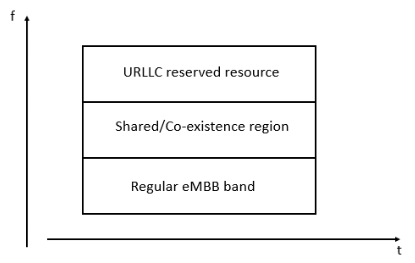
\includegraphics[scale=0.35]{fig4.png}}
\caption{Semi-static resource sharing.}
\label{fig4}
\end{figure}

In semi-static resource sharing, there are the regions that are exclusive to eMBB or URLLC transmissions. Because URLLC traffic might be sparse, the eMBB UEs are able to be configured to transmit in one part of URLLC band. This band is called a shared/co-existence region. When the eMBB UEs are allocated transmission resource in the only-eMBB band, it is certain that there is no collision with the URLLC UEs. Thereby, the gNB does not need to activate these UEs to increase monitoring periodicity in order to listen to PI.

In contrast, if the eMBB UEs are configured to transmit in the shared region, there is a chance that the gNB must stop their transmission to prioritize URLLC transmission. These eMBB UEs are required to listen to PI in mini-slot level so that they can stop their transmission in the shortest delay.

\textbf{Proposal 1: Only the eMBB UEs scheduled to transmit in the shared region of semi-static are triggered by the gNB to increase monitoring periodicity and listen to PI in mini-slot level.}

\textbf{\underline{Multiplexing between eMBB GB and URLLC GB transmission}}

When the gNB sends PI to the eMBB UE to stop the scheduled transmission and avoid an interference with the URLLC UE, not all the eMBB UEs are the candidates for a cancellation of transmission. One example is shown in Fig.~\ref{fig2}, the gNB chooses the eMBB UE 2 to become a candidate for a potential cancellation based on its data size. The eMBB UE 2 has a smaller packet than the eMBB UE 1 so the gNB consumes less resources for a retransmission after cancelling its transmission. In addition, the eMBB UE 1 with a larger packet size has more chance to have collision with a URLLC UE. This means that it might have to stop or puncture data many times and there is a higher probability that the packet is not decoded correctly.

For this reason, only the eMBB UE 2 that has been chosen by the gNB for a potential data cancellation if there is a need of the URLLC UE must listen to PI. Thus, only this UE has to increase its monitoring periodicity for PI monitoring in mini-slot level. The gNB triggers this increase when it chooses the eMBB UE candidates for cancellation.

\textbf{Proposal 2: Only the eMBB UEs that are chosen as candidates for potential cancellation by the gNB are triggered to increase monitoring periodicity.}

Another way to choose the UE candidates is based on the UE capability. Not all eMBB UEs are able to listen to DCI in mini-slot so these UEs are not chosen to stop the transmission in the overlapping region because it might not be likely to stop the transmission in short delay to satisfy URLLC latency requirement.

The positions of the eMBB UEs are also taken into account. The UEs at the edge of cell are not chosen for potential cancellation because these UEs use higher power and lower MCS for the initial transmission to achieve the requirement so much more power and resources are needed for a retransmission than the UEs being near to the gNB. Channel condition that the gNB knows from SR is also a criterion to choose UE candidate for cancellation.

\textbf{Proposal 3: The eMBB UE candidates are chosen based on selection criteria following the order: UE capability, UE position to the gNB, data size and channel condition.}

The basic idea here is that the base station can apply some selection rules on the transmissions so that to limit the eMBB UEs that it may pre-empt in case of some urgent URLLC transmission needs to be scheduled. One simple example was discussed that a UE which is scheduled large transport block (TB) is not be pre-empted compared to a user which shorter TB if its pre-emption allows the base station to handle the URLLC requirements.

\textbf{\underline{Multiplexing between eMBB GB and URLLC CG transmission}}

If the eMBB data overlaps the CG regions, the eMBB UEs transmitting this data have to increase monitoring periodicity to listen to PI in mini-slot level because URLLC data may come without the gNB’s knowing. The eMBB UEs are demanded to stop by the gNB if there is an URLLC UE who also transmit in the scheduled CG region. The cancellation of eMBB transmission helps to protect the retransmission of the URLLC UE in the next CG region.

\textbf{Proposal 4: The eMBB UEs are triggered by the gNB to increase monitoring periodicity when they are allocated resources in the CG regions.}

\subsubsection{Mechanism to activate an increase of monitoring periodicity}

If the eMBB UEs are configured to monitor PI in mini-slot level all the time after being scheduled, power consumption would rise significantly. Therefore, only the eMBB UEs specified in Proposal 1, Proposal 2, Proposal 4 are triggered to increase monitoring periodicity. This activation is done by the gNB when it includes 1-bit flag in the UL grant to help the eMBB UEs perceive their situation and do monitoring in mini-slot level. The bit used as a flag can be a padding bit or the first bit in the field of frequency domain resource assignment.

\textbf{Proposal 5: 1-bit flag is used in the UL grant of the specific eMBB UEs to make them realize their situation and trigger an increase of monitoring periodicity. This bit can be a padding bit or the first bit in the field of frequency domain resource assignment.}

\subsubsection{Limit of monitoring periodicity for eMBB UEs}

An increase of monitoring periodicity can be carried out without a big modification in the UE design. In 5G NR, the UE supports different sub-carrier spacing (SCS): 15 kHz, 30 kHz, 60 kHz, 120 kHz.

\begin{figure}[htbp]
\centerline{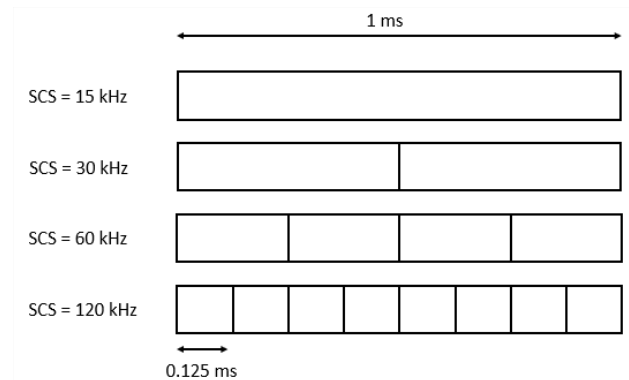
\includegraphics[scale=0.35]{fig5.png}}
\caption{SCS terminology.}
\label{fig5}
\end{figure}

In 1 ms, the maximum number of slots are 8 slots with SCS 120 kHz. If the UEs monitor DCI in slot level, they have 8 monitoring occasions. This means that the UEs are already capable of supporting 8 monitoring occasions with their current design. Therefore, it is proposed that the number of monitoring occasions are still kept the same at 8 occasions in 1 ms even if the value of SCS decreases after the eMBB UEs receive 1-bit flag in UL grant. This value allows the eMBB UEs to monitor PI in mini-slot level when a low SCS is used. Normally, with SCS 60 kHz, there are only 4 monitoring occasions in 1 ms. However, with this proposal, the number of occasions are doubled to 8. At this moment, the UEs monitor DCI in non-slot level at each interval of 0.125 ms. The impact of this proposal is even bigger for low SCS 15 kHz and 30 kHz.

\textbf{Proposal 6: When an eMBB UE is indicated to decode sub-slot level pre-emption indication, it can be configured to DCI Periodicity going up to its highest capability sub-carrier spacing slot timing. As an example, if a UE is capable of operating at 120 KHz SCS, and is currently operating at 15 KHz SCS, it can be configured to decode pre-emption indication DCI upto 120/15 = 8 distinct time occasions within a slot.}

Monitoring capability also have to be enhanced if monitoring occasions increases, especially for SCS 15 kHz. In normal case, the UEs have 44 PDCCH candidates and 56 non-overlapped CCEs in a 1ms-slot with SCS 15 kHz. When the number of occasions grow to 8 in 1ms-slot, the UEs only have around 5 PDCCH candidates and 7 CCEs for each monitoring occasion. If an AL 8 is required for PI so as to guarantee the reliability, there are not enough CCEs for that PI. Due to the very high reliability of URLLC transmission, the reliability of PI to stop the eMBB transmission is also high and approximate to the requirement of URLLC (10\textsuperscript{-5}). The maximum number of CCEs should be kept the same at 64 CCEs for all SCS to ensure that PI is bound to be transmitted with AL 8. Similar to the proposal of the value of monitoring occasions, this maximum number of CCEs are only applied after the eMBB UEs receive an indication of 1 bit-flag in UL grant.

\textbf{Proposal 7: The maximum number of CCEs should be kept the same at a value to guarantee mini-slot monitoring for all SCS after the eMBB UE receives an indication by 1 bit-flag in UL grant to monitor PI in mini-slot level.}

The number of monitoring occasions that an URLLC UE are able to increase can be defined by different criteria than SCS as in Proposal 6. Based on the processing time of DCI, the eMBB UE can define the maximum number of occasions that it can monitor and decode blindly DCI.

\textbf{Proposal 8: The maximum number of monitoring occasion can be defined by other featured rather than SCS as the processing time of DCI in each occasion.}

\subsubsection{Period of monitoring occasion}

URLLC transmission is carried out in mini-slot level with period of 2, 4 and 7 symbols for normal prefix or 2, 4, 6 symbols for extended prefix. The eMBB UEs are demanded to monitor PI in the same period of URLLC transmission so they can realize the overlapping situation indicated by the gNB and stop their transmission in the shortest delay. This means that monitoring occasions increase from 1 per slot to 7, 4 and 2 corresponding to period of 2, 4 and 7 symbols of URLLC transmission for normal prefix or 7, 4 and 3 corresponding to period of 2, 4 and 6 symbols of URLLC transmission for extended prefix.

The requirement of monitoring periodicity can be relaxed and larger than the scheduling transmission level of URLLC if the traffic is not much sensitive to latency. Another possibility is if processing time of PI at the eMBB UE is much faster than processing time of UL grant at the URLLC UE who also transmits in the GB region. It is a feasible possibility because the eMBB UE only needs to proceed PI and stops transmission while the URLLC UE must consume much time in decoding UL grant and preparing data for the uplink transmission.

\subsubsection{UL overlap avoidance indication for URLLC UEs}

As proposed in R1-1812225, When the gNB allocates resources for the eMBB UEs on both grant-based (GB) and configured grant (CG) region, CG URLLC transmission may collide with eMBB transmission because the gNB does not know URLLC transmission in advance by SR. A signal is sent by the gNB to the URLLC UEs at the same time with the UL grants of the eMBB UEs to warn the URLLC UEs about a presence of eMBB transmission in the CG region as shown in Fig.~\ref{fig6}.

\begin{figure}[htbp]
\centerline{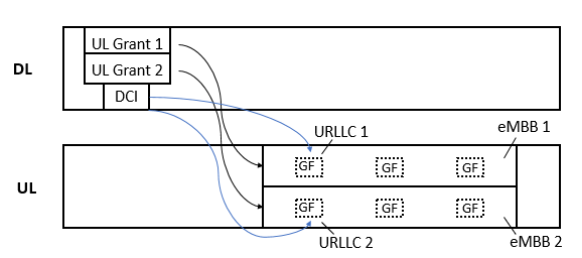
\includegraphics[scale=0.35]{fig6.png}}
\caption{Signalling the URLLC UEs about an overlap with the eMBB UE in the configured grant region.}
\label{fig6}
\end{figure}

Our disclosure proposes the behaviour of the URLLC UEs when they receive a signal warning about an overlap in the CG region in order to avoid a collision with the eMBB transmission. 

Upon decoding the signal from the gNB, the URLLC UEs know which CG regions have been taken by the eMBB UEs. The URLLC UEs are able to choose one of the following ways depending on latency and available resources to avoid and reduce the collision with eMBB transmission so the strict requirements will be satisfied.

\begin{figure}[htbp]
\centerline{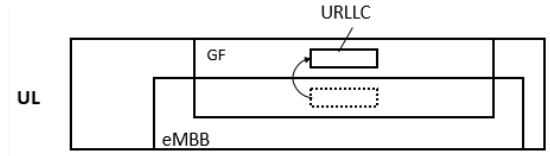
\includegraphics[scale=0.35]{fig7.png}}
\caption{URLLC moves to available CG region in the same time interval.}
\label{fig7}
\end{figure}

In the first case, if the eMBB data only overlaps a part of the CG region as illustrated in Fig.~\ref{fig7}, the URLLC UEs move to the available resource of the same CG region if the resource is enough for URLLC data. In Release 15 of 3GPP, the CG users are configured with resource size, transport block size and MCS among other CG parameters.  This means that normally as soon as part of the resource becomes unavailable, they can not transmit the configured transport block size with the configured MCS. To handle this case, the proposal would be to allow the UE to choose a suitable MCS for the configured transport block size. This way, the user would be able to adjust its transmitted data to fit the remaining non-overlapping resources in the CG region. As the gNB has indicated the overlapping region to the URLLC UE, it also does the same calculation to find the suitable MCS and thus, it knows which MCS the URLLC UE would choose to send in this partially overlapping CG resource.

\textbf{Proposal 9: When the eMBB resources partially overlap with the CG region, the URLLC UE transmits data in the CG part that are not overlapped by adapting a suitable MCS indicated by the gNB through a DCI signal.}

\begin{figure}[htbp]
\centerline{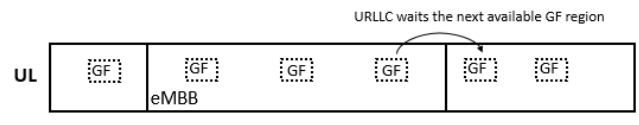
\includegraphics[scale=0.35]{fig8.png}}
\caption{URLLC waits the next available CG region.}
\label{fig8}
\end{figure}

In the second case, if the eMBB data overlaps an entire CG region as in Fig.~\ref{fig8}. The URLLC UE senses latency budget to decide whether it has enough time to wait for the next available CG region. It has information about the CG regions in the next occasion that have not been taken by the eMBB UEs by decoding the signal from the gNB. If latency budget is enough, the URLLC UEs wait for a non-overlapping CG region to avoid interference with the eMBB transmission.

\textbf{Proposal 10: When the eMBB resources fully overlap with the CG region, the URLLC UE waits for the next non-overlapping CG region if latency budget is sufficient.}

\section{Two-step strategy in eMBB and URLLC multiplexing}\label{Ap2}
\subsection{Introduction}

One main target of the 5G New Radio (NR) standard is to support URLLC for devices requiring low latency and high link reliability. In \cite{ad1}, The 3rd Generation Partnership Project (3GPP) defines targets for the URLLC scenario: ``A general URLLC reliability requirement for one transmission of a packet is 10\textsuperscript{-5} for 32 bytes with a user plane latency of 1 ms''. The next release of 3GPP will have higher requirements of URLLC: ``Higher reliability (up to 10\textsuperscript{-6}), higher availability, short latency in the order of 0.5 to 1 ms, depending on the use cases (factory automation, transport industry and electrical power distribution)''\cite{ad2}.

\subsubsection{Techniques accepted in 3GPP Release 15}\label{B11}

3GPP Release 15 specified new features in physical layer design to help URLLC achieve its requirements.

Subcarrier spacings (SCS) has a flexible range from 15 kHz to 240 kHz in 5G that results in very short symbol and slot timings\cite{ad6}. In addition, the transmission is scheduled in  mini-slot level in both UL and downlink (DL)\cite{ad7}. Due to these features, the network becomes very reactive to UEs' UL and DL traffic demands and the response time to accommodate DL or UL traffic is very small compared to Long-Term Evolution (LTE) and LTE-Advanced.

Another feature is the standardization of the CG/CG UL transmissions which allows the UEs to transmit data in UL without having to transmit an explicit SR and receiving an UL grant to reduce latency \cite{ad3}.

\subsubsection{Problem of multiplexing URLLC and eMBB in CG resources}

In 5G, as mentioned in Section \ref{B11}, the gNB can schedule CG resources for URLLC UEs but it does not have any prior information which of these CG resources will actually be used by URLLC UEs or which of the UEs in the group configured to the resources will use a specific resource. If the cell is loaded and the gNB schedules some eMBB UEs on the resource overlapping with CG occasion, as shown in Fig.~\ref{fig11}, there is going to be transmission collision of dynamically scheduled eMBB and URLLC CG transmissions. 

\begin{figure}[htbp]
\centerline{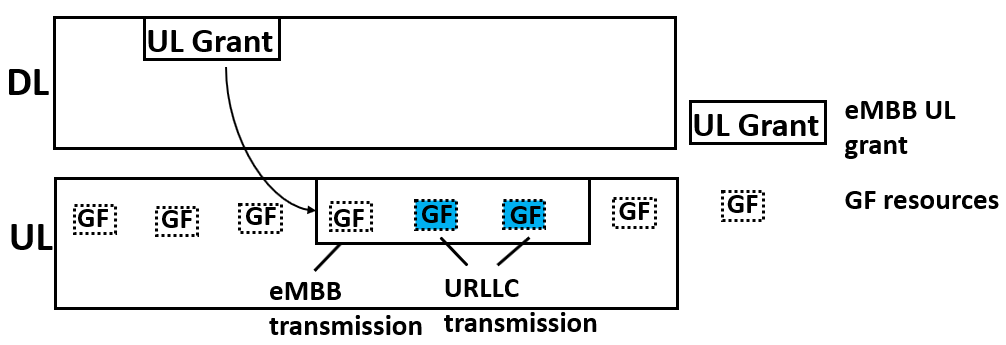
\includegraphics[scale=0.35]{fig11.PNG}}
\caption{A collision of UL URLLC CG transmission with eMBB transmission in case of Frequency Division Duplex (FDD).}
\label{fig11}
\end{figure}

When the transmissions from eMBB and URLLC UEs in CG resources overlap, it results in lower decoding probability due to lower resulting SINR for both UEs. This can be a serious problem for URLLC UEs in particular due to their tight latency and reliability targets.

In case the gNB is able to identify the URLLC UE from its DMRS sequence, it may try to quickly reschedule the UE over non-overlapping resources if an error happens.

The increased interference due to overlapping transmissions of eMBB and URLLC UEs may lead to a catastrophic situation when the gNB may not even identify the URLLC UE (DMRS miss-detection). The current HARQ structure in UL transmission for NR is timer based, which means that upon transmission of packet, the UE will start the HARQ timer. If it receives an UL grant for the re-transmission of the same transport block (TB) from the gNB, it does the retransmission over the resources scheduled in the UL grant. If it receives no UL grant from the gNB and the HARQ timer expires, it considers that the TB was successfully decoded at the gNB and discards the data in the buffer. 

The timer-based HARQ feedback and UL GB retransmission are standardized because this minimizes the control overhead for sending HARQ feedback. This is reasonable in general but in the cases of dynamic UL multiplexing, giving rise to overlapping transmissions with CG UEs, when the gNB will not be able to identify the UEs transmitting on CG resources, the UEs will discard their packets and consider the successful detection that leads to serious performance degradation for URLLC UEs.

\subsubsection{Prior art}
In \cite{ad8} and \cite{ad9}, when there is an overlap, the gNB asks the URLLC UE to apply a different pre-configured transmission power that is higher than power level used in case of no overlap. However, an increase of power causes an interference among the neighboring cells. Secondly the cell-edge UEs may be power limited and cannot raise their transmission power. This is also the problems of \cite{ad10} when the gNB assigns URLLC physical uplink shared channel (PUSCH) with updated transmission parameters such as resource, MCS, transmit power, etc. on CG resources that are occupied by eMBB PUSCH. 

In \cite{ad11}, the group common control channel reveals resource range allocated to GB eMBB UE so the CG UE can exclude the occupied resource. Nevertheless, the CG UE has less resources left to transmit than the original configured resources so this partial transmission may not be decodable at the gNB.

In \cite{ad12}, the gNB informs the URLLC UE which of the CG resource set has overlapping eMBB transmission such that the URLLC UE can initiate the CG transmission over resources not occupied by the ongoing eMBB transmission. It might result in high latency if all resources in the current occasion are full and the UE must wait until the next transmission occasion.

A preemptive scheme in \cite{ad13} cannot be applied in URLLC CG transmission because the gNB does not know the URLLC transmission in advance to preempt eMBB transmission.

A successive interference cancellation (SIC) receiver in \cite{ad14} only benefits eMBB UE rather than URLLC UE because URLLC data is decoded first due to latency requirement.

In this work, a multiplexing scheme with two-step strategy is presented in Section \ref{B2}. The first step comprises of the gNB transmitting an overlap indication whenever it schedules an UL transmission having an overlap with the resources configured to the CG transmissions. The second step of the proposed strategy comprises of making the overlapped transmissions to use explicit HARQ feedback structure. An alternative way of the second step is to make the gNB indicate the UEs to send SR in parallel to data transmitted on the CG resources to improve the reliability. Section \ref{B3} shows numerical results and performance evaluation. Finally, Section \ref{B4} is conclusion.

\subsection{Strategy to multiplex the eMBB and URLLC UEs}\label{B2}

\subsubsection{Overlap indication and explicit HARQ acknowledgement (ACK) feedback}\label{B21}

This paper proposes two-step strategy to overcome the problem of the multiplexed UL eMBB and URLLC transmissions. In the first step, upon scheduling a GB transmission of the eMBB UE over the CG resources, the gNB sends an indication of resource overlap to the URLLC UEs. As the gNB does not know which of the URLLC UEs configured for CG resources may become active in the current interval, this indication needs to be sent to all UEs who have been configured with the CG resources in the overlapping interval as illustrated in Fig.~\ref{fig12}. Upon receiving this overlap indication, the URLLC UEs are aware of the resources which have been dynamically scheduled for other UEs and in case of transmission,  their transmissions will be received with an increased interference.

\begin{figure}[htbp]
\centerline{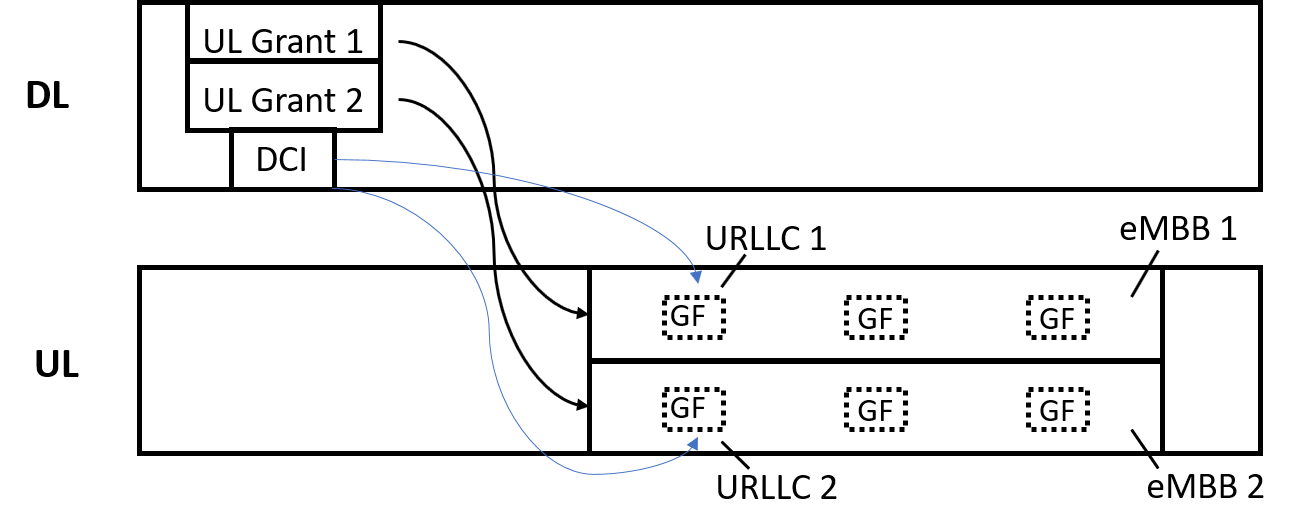
\includegraphics[scale=0.35]{fig9.png}}
\caption{Signalling the URLLC UEs about an overlap with the eMBB UEs in CG regions.}
\label{fig12}
\end{figure}

The second step of the proposed strategy comprises of making the overlapping transmissions use explicit HARQ feedback structure rather than legacy timer-based feedback. The resource overlap indication can serve this purpose by containing a 1-bit flag to tell if the feedback becomes explicit or not. Upon receiving this indication, the URLLC UEs, who transmit on the overlapping resources, expect to receive explicit HARQ feedback from the gNB for their transmissions. 

Thereby, within a configured time period, the CG UEs receive either explicit HARQ ACK indicating the successful detection of their TB or UL grant for re-transmission in case the gNB failed to decode the TB but was able to identify the transmitting UE.  For the third case, if the gNB even fails to identify the UE due to high interference (DMRS miss-detection), it cannot schedule the UE for a re-transmission in the conventional timer-based feedback so the UE assumes that a packet is decoded correctly and drops it from buffer to transmit the next packet. This is the scenario where our proposed explicit HARQ feedback becomes the most promising. If the CG UE receives neither an ACK nor an UL grant within a configured time, the UE does not consider that its data is successful, rather it considers that the gNB failed to identify its identity (ID) due to high interference in the overlapping transmissions and retransmits the TB on the subsequent CG resources. Table~\ref{tab3} summarizes the operation of conventional timer-based feedback structure and explicit feedback structure.

\begin{table}[htbp]
\caption{Comparison of different feedback structures}
\begin{center}
\begin{tabular}{|p{8em}|p{7em}|p{7em}|}
 \hline
 \textbf{Case} & \textbf{Timer-based feedback}&\textbf{Explicit feedback}\\
 \hline
 DMRS: detected&No ACK/UL grant&ACK\\TB: decoded & &\\
 \hline
  DMRS: detected&UL grant: &UL grant:\\TB: failed & reschedule&reschedule\\
 \hline
DMRS: failed&No ACK/UL grant: packet lost&No ACK/UL grant: packet retransmitted auotmatically\\

%  increase row height, number of & = number of collumn
% &&&&&\\[-1em]
 
 \hline
\end{tabular}
\label{tab3}
\end{center}
\end{table}

Block error rate (BLER) of a packet in timer-based feedback structure and explicit feedback structure is shown in \eqref{eq1} and \eqref{eq2} in Section \ref{B3}.

The timer value, for which the UE should wait to receive ACK or UL grant, can be configured by radio resource control (RRC) parameters. This value can be selected as a function of reliability and latency targets of the UEs. For some UEs with extremely high latency and reliability targets, this timer value can be put to zero which means to do the automatic transmission in case of overlapping transmissions to maximize the chance of correct data detection at the gNB.

\subsubsection{Overlap indication and additional SR}\label{B22}

In a variation of the proposed scheme in Section \ref{B21}, the second step of making the transmissions explicit HARQ feedback-based can be replaced to use an additional SR. The gNB can indicate the URLLC CG UEs by overlap indication in the first step described in Section \ref{B21} to send a SR in parallel for the TB transmitted over the overlapping CG resources. The SR sent to the gNB will provide a further means besides DMRS detection to detect the ID of the UE transmitting in the interfered CG transmission. When the gNB is unable to identify the UE making the CG transmission because of DMRS miss-detection, the gNB still can identify that UE by decoding the additional SR and react fast to the received SR by sending an UL grant to this UE. Thanks to the UL grant, the UE is likely to retransmit the packet and has a successful transmission in latency budget instead of assuming a succesful transmission and dropping the packet as in the conventional scheme. When the gNB is able to decode the data successfully, it still reacts to SR to send some indications to the UE about the successful detection.  

Physical uplink control channel (PUCCH) and PUSCH are not allowed to be transmitted simultaneously. In case the UE needs to transmit uplink control information (UCI) while transmitting UL data on PUSCH, it sends the UCI on PUSCH. When the UE is not transmitting PUSCH, it sends the UCI carrying SR, feedback for DL data  etc, on the PUCCH resources using appropriate PUCCH format as a function of UCI content and the PUCCH configurations. The simplest strategy to send SR (which is UCI) when the URLLC UE is transmitting over overlapping CG resources would be to transmit it over PUSCH CG resources along with the transmission of the TB. This can be simple from implementation perspective but from the performance point of view, it does not help to improve significantly the performance of the UE ID detection. If DMRS of PUSCH is not detected by the gNB because of bad channel and interference from eMBB transmission, there is high chance that the gNB also cannot decode the SR to obtain the UE ID multiplexed with PUSCH. For this reason, to achieve a better UE ID detection, the SR is proposed to be transmitted using PUCCH configuration on the specified PUCCH resources separated from PUSCH. As PUCCH resources are dedicated resources on different frequency physical resource blocks (PRBs) and OFDM symbols, this provides additional diversity advantage to the SR transmitted in these resources compared to multiplexing and transmitting it over UL CG resources along with the TB. Therefore, the UE is configured to transmit this SR on PUCCH resources in parallel to the transmission of TB on the overlapping resources.

The overlap indication may have an explicit indication, in the form of a single bit flag, which may require the UEs transmitting over overlapping CG occasions to send SR. In fact, more flexibility and better performance can be achieved by having the flexible control of the explicit HARQ feedback structure and the transmission of SR. The gNB can then choose which strategy to choose in different situations. As an example, if the periodicity of current CG occasions is not very fast, it may make sense to indicate the overlapping CG UEs to send an SR. And in the cases, if the resources configured for SR are not sufficient or not in close proximity compared to the subsequent CG occasions, it may be suitable to prioritize the explicit HARQ feedback and automatic retransmission in case the UEs receive no ACK/UL grant indication for the transmitted TB.

\subsubsection{Configuration and Signalling for the Overlap Indication}

One very important feature of the proposed scheme is that the overlap indication is sent to the UEs who have been pre-configured for the CG resources. As CG resources may be shared by multiple UEs, and the gNB has no idea a priori which of these UEs may transmit their data over CG resources, this overlap indication is sent in a group-common manner. Thus, the proposal is to send the overlap indication in a group-common downlink control information (DCI).

For UL overlap indication sent in group-common DCI, a DCI format similar to the DCI format 2\_1 in \cite{ad15} can be used. DCI 2\_1 is also used for DL pre-emption indication. The size of DCI format 2\_1 is configurable by higher layers up to 126 bits and each indication has 14 bits. 

The UL overlap indication sent to the URLLC UEs comprises of the indication of UL CG resources typically scheduled for the eMBB UEs. The eMBB UEs would be normally scheduled for the slot duration or most part of the valid UL symbols so it would be judicious to have more bits of UL reference resource field defining the frequency granularity. To keep a format close to the DL pre-emption indication and adapted to indicate the UL overlap resource, there are two possibilities of UL overlap indication. In the first design, all 14 bits are used to indicate the frequency PRB region for the whole slot. Thus, each bit in the 14-bit long bitmap indicates 1/14 of the frequency PRBs of the carrier as shown in left part of Fig.~\ref{fig13}. The second option is to split the time-frequency grid of the slot in 7 frequency zones each spanning one half slot. Thus, each bit may indicate an overlap over 1/7 of the frequency PRBs for a half slot time duration as illustrated in right part of Fig.~\ref{fig13}. 

\begin{figure}[htbp]
\centerline{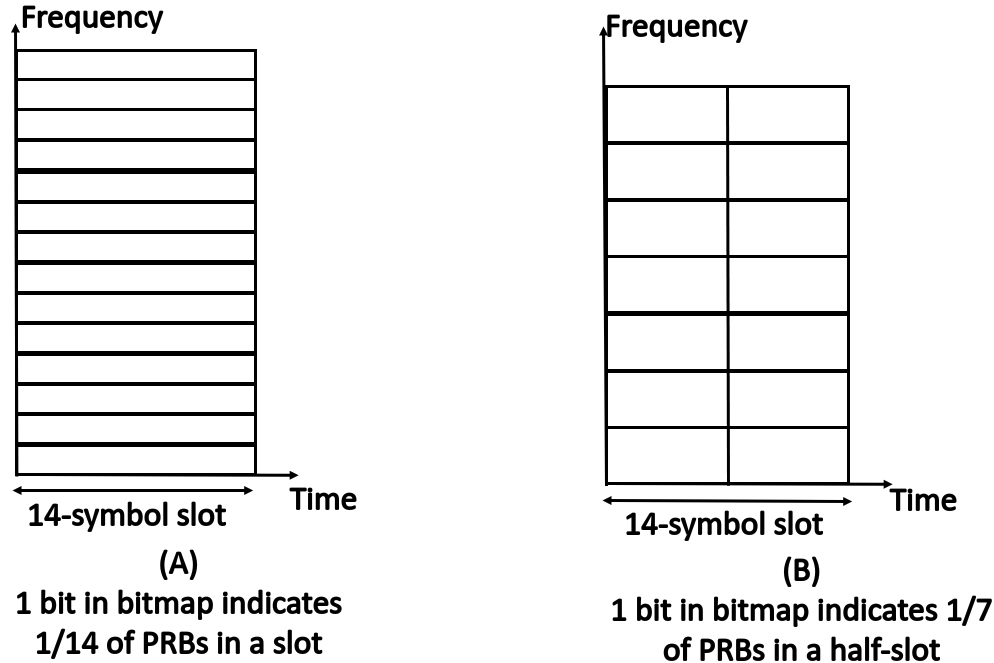
\includegraphics[scale=0.3]{fig13.png}}
\caption{Resource Indication in Uplink Overlap Indication.}
\label{fig13}
\end{figure}

The UEs configured with CG resources can be configured to listen and decode the overlap indication as part of CG configuration. The activation or de-activation of this operation can be done in different ways for Type 1 and Type 2 CG as specified in \cite{ad6}. For RRC configured Type 1, the activation and de-activation can be done by RRC signalling. For configured grant Type 2, where some parameters of CG can be updated by DCI, the activation or de-activation of overlap indication can be made through DCI signalling which is used to update other CG parameters.

The overlap indication can be sent at the same time when the gNB sends the dynamic UL grant scheduling a UE over the CG resources as shown in the left part of Fig.~\ref{fig14}.

When the gNB sends an UL grant scheduling an eMBB UE, the scheduled resources are not necessarily in the same slot where UL grant is sent. Rather typically the UL grant will be for the resources located in one of the subsequent slots. If the gNB transmits the overlap indication along with the UL grant, it needs to indicate the slot where this overlap will occur. To avoid this additional signalling and to keep the treatment of UL grant simple, the overlap indication can be transmitted in the slot where overlap occurs as shown in the right part of Fig.~\ref{fig14}. However, it may not be preferable to send and receive at the same time, so transmitting the overlap indication in the DL direction in the same slot as of the overlapping CG occasions may not be very interesting. In some other cases like time division duplex (TDD) operation mode, it may be completely impossible. Thus, based on the system design, one of these two transmission schemes
is determined.

\begin{figure}[htbp]
\centerline{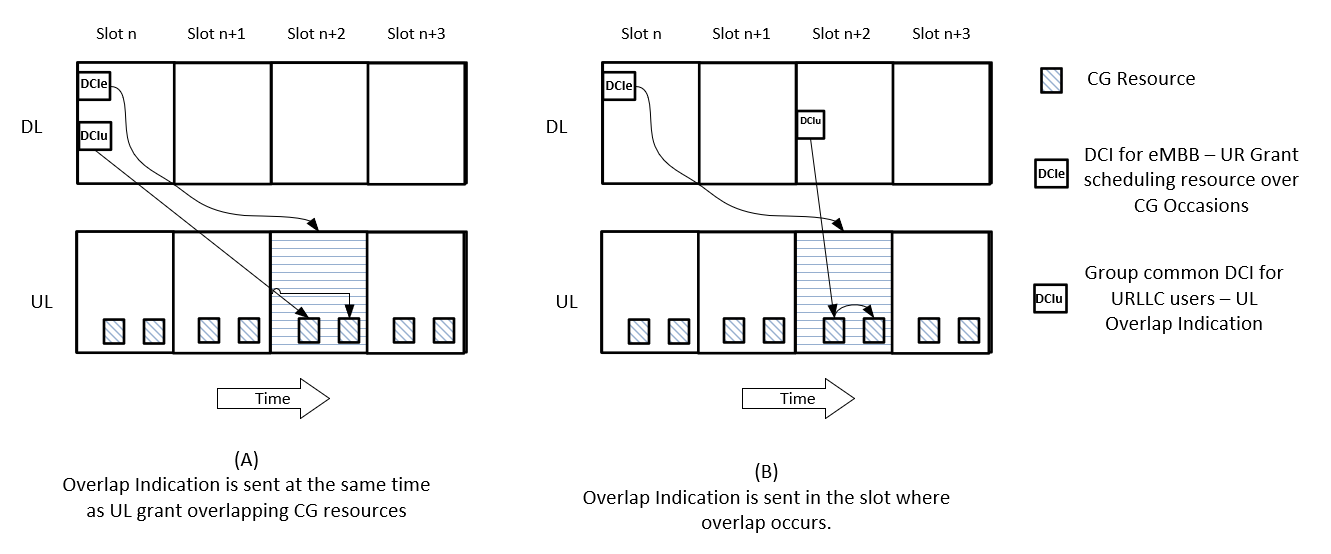
\includegraphics[scale=0.3]{fig14.png}}
\caption{Timing to send the UL Overlap Indication.}
\label{fig14}
\end{figure}

One big advantage of sending the overlap indication to URLLC UEs is that the overlap indication is primarily indicating the overlap caused by dynamic scheduling of eMBB UEs over the CG resources. As eMBB UEs may be scheduled only once during a slot, the indication periodicity can be kept to be once per slot and no mini-slot monitoring is needed to receive the overlap indication. This is advantageous in the sense that it does not overload the UEs with additional DCI monitoring and decoding burden.

\subsubsection{Design of Explicit HARQ Feedback}
In the proposed strategy, the gNB shifts the CG transmissions in the overlap region from timer-based approach to explicit-HARQ-feedback approach. Thus, a design for the explicit HARQ feedback in general may be needed. The proposal is to use DCI as an explicit HARQ feedback sent with UE specific configured scheduling-radio network temporary identifier (CS-RNTI) which is used with configured grant-based transmissions. If the gNB is able to successfully decode the data despite the overlap, it can send an UL grant to this UE with the same HARQ process number (HARQ ID) as of the successfully received TB, and the UE upon receiving this UL grant would know that this is in fact not a retransmission request but an explicit ACK for the previously transmitted TB. To avoid any confusion, new-data-indicator (NDI) field can be set to zero. Further, some of the fields in the DCI which are actually not needed, such as the time and frequency resource assignment fields, may be sent with fixed known values which can be pre-decided to be used in the ACK indication.

\subsection{Numerical results and performance evaluation}\label{B3}



Simulation parameters are shown in Table~\ref{tab4}. Fig.~\ref{fig15} illustrates the performance of DMRS detection in three cases: the URLLC UE transmits in the CG resources without any collision with another eMBB UE, the URLLC UE has a collision with an eMBB UE at the same power level and the URLLC UE has a collision when increasing power 1dB higher than an eMBB UE. For each DMRS detection, the correlation result is compared with a threshold to determine whether DMRS exists or not. This threshold is chosen according to a target false alarm rate (FAR) indicating the cases that the gNB determines the existence of DMRS while in reality there is no DMRS transmitted. A higher threshold is required for a lower FAR but also results in more missed detection.

\begin{table}[htbp]
\caption{Simulation parameters}
\begin{center}
\begin{tabular}{|p{8em}|p{8em}|}
 \hline
 \textbf{Parameters} & \textbf{Values}\\
 \hline
 Waveform & CP-OFDM\\
 \hline
 Subcarrier spacing & 60kHz\\
 \hline
 Channel model & Rician\\
 \hline
 K factor & 1\\
 \hline
 Number of allocated PRB & 8\\
 \hline
 DMRS detection mechanism & Time-domain correlation\\
 

%  increase row height, number of & = number of collumn
% &&&&&\\[-1em]
 
 \hline
\end{tabular}
\label{tab4}
\end{center}
\end{table}

\begin{figure}[htbp]
\centerline{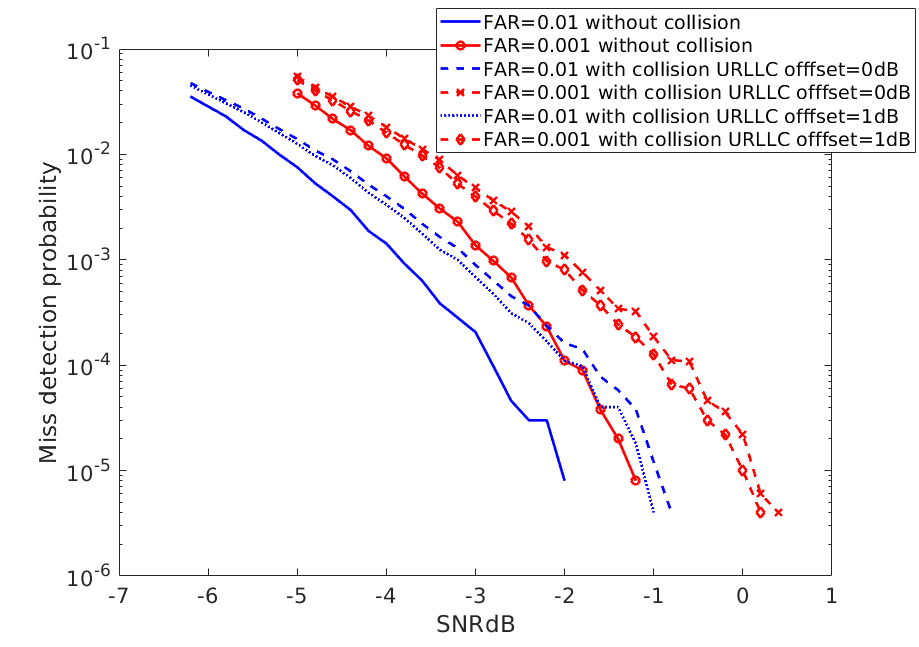
\includegraphics[scale=0.33]{fig10.png}}
\caption{DMRS detection performance.}
\label{fig15}
\end{figure}

Due to a collision between DMRS of the URLLC UE of interest and data/DMRS of another eMBB UE, the performance of DMRS detection of the URLLC UE degrades significantly as can be seen in Fig.~\ref{fig15} and cannot achieve the miss detection probability 10\textsuperscript{-5} at the same SNR level of the case without collision. At FAR of 0.001 and SNR of -1.4dB, the miss detection probability increases from 10\textsuperscript{-5} of the case without collision to 3.4$\times$10\textsuperscript{-4} of the case with a collision with an eMBB UE at the same power. Fig.~\ref{fig15} also shows that even with power control scheme in \cite{ad4} and \cite{ad5} when the URLLC UE's power increases 1dB higher than the eMBB UE's power, miss detection probability is still 2.44$\times$10\textsuperscript{-4} that is higher than 10\textsuperscript{-5} of the case without collision. As DMRS dectection is mandatory for channel estimation to decode data as well as for recognizing UE ID to reschedule a retransmission if necessary in conventional scheme, a degradation of DMRS detection makes the system unable to support reliability URLLC requirement. BLER of an UL transmission with one potential retransmission in the conventional scheme or power control scheme ($ P^{e}_{1}$) is calculated as\useshortskip

\begin{equation}
\begin{split}
 &P^{e}_{1} = P^{e}_{DMRS1} + \\
        &+ (1-P^{e}_{DMRS1})P^{e}_{d1}(P^{e}_{DMRS2} + (1-P^{e}_{DMRS2})P^{e}_{d2}),\label{eq4}   
\end{split}
\end{equation}
where $ P^{e}_{DMRS1}, P^{e}_{DMRS2}$ are the miss detection probabilities of the initial (with collision) and retransmitted (without collision) DMRS (see Figure \ref{fig15}), and $P^{e}_{d1}, P^{e}_{d2}$ are the error probabilities of the initial (with collision) and retransmitted (without collision) PUSCH.

In \eqref{eq4}, the first term is the error probability when the gNB cannot detect DMRS to decode or reschedule data so the UE does not retransmit data and data is lost. The second term is the error probability when the gNB detects DMRS and indentifies UE ID but fails to decode data so it reschedules data. However, it cannot decode the retransmission and an error still occurs.

The usage of an explicit HARQ feedback as explained in Section \ref{B21} solves the problem of DMRS miss-detection in the overlapping region because it allows the UE to carry out the retransmissions in the interference-free regions even if DMRS is not detected by the gNB. BLER of an UL transmission with one potential retransmission in the proposed scheme with explicit feedback ($ P^{e}_{2}$) is calculated as\useshortskip

\begin{equation}
\begin{split}
 &P^{e}_{2} = P^{e}_{DMRS1}(P^{e}_{DMRS2} + (1-P^{e}_{DMRS2})P^{e}_{d2}) + \\
        &+ (1-P^{e}_{DMRS1})P^{e}_{d1}(P^{e}_{DMRS2} + (1-P^{e}_{DMRS2})P^{e}_{d2}).\label{eq5}   
\end{split}
\end{equation}

Compared to \eqref{eq4}, the first term in \eqref{eq5} is enhanced because of a retransmssion while the second terms are the same.

\begin{table}[htbp]
\caption{Performance comparison between different scenarios and schemes at SNR=$-1.4dB$, FAR=0.001, $P^{e}_{d2}$=$P^{e}_{SR}$=0.01}
\begin{center}
\begin{tabular}{|p{14em}|p{7em}|p{10em}|p{10em}|}
 \hline
 \textbf{Case} & \textbf{URLLC UE ID miss detection probability}& \textbf{Retransmission in UE ID miss detection}& \textbf{URLLC UL transmission's BLER due to the first UE ID miss detection}\\
 \hline
 No collision  & 10\textsuperscript{-5}&No&10\textsuperscript{-5}\\
 \hline
 Collision in the conventional scheme& 3.4$\times$10\textsuperscript{-4}&No&3.4$\times$10\textsuperscript{-4}\\
 \hline
 Collision with power control (\cite{ad4} and \cite{ad5})&2.44$\times$10\textsuperscript{-4}&No&2.44$\times$10\textsuperscript{-4}\\
 \hline
 Collision with explicit feedback (proposed)& 3.4$\times$10\textsuperscript{-4}&Yes&3.4$\times$10\textsuperscript{-6}\\
\hline
 Collision with additional SR (proposed)& 3.4$\times$10\textsuperscript{-6}&No&3.4$\times$10\textsuperscript{-6}\\

%BLER_trans=P_DMRS+(1-P_DMRS)*P_data
%  increase row height, number of & = number of collumn
% &&&&&\\[-1em]
 
 \hline
\end{tabular}
\label{tab5}
\end{center}

\end{table}

The final column in Table~\ref{tab5} shows a remarkable enhancement of the first term of error probability in UL transmission with explicit HARQ feedback in case of URLLC and eMBB multiplexing in comparison to the conventional scheme with timer-based feedback and power control scheme in \cite{ad4} and \cite{ad5}. Moreover, the proposed scheme can be applied to all UEs in a cell while the power control scheme to increase URLLC UEs' power cannot be applied to the cell-edge UEs because of power limitation. 

Table~\ref{tab5} also shows an improvement of UE ID detection (the first term in \eqref{eq6}) when an additional SR is transmitted in the separate PUCCH in parallel with data (PUSCH) in CG resources. As can be seen in \eqref{eq6}, the SR provides another chance for the gNB to detect UE ID. Therefore, the error probability because of DMRS miss-detection decreases. BLER of an UL transmission with one potential retransmission in the proposed scheme with an additional SR ($ P^{e}_{3}$) is calculated as\useshortskip

\begin{equation}
\begin{split}
 P^{e}_{3} &= P^{e}_{DMRS1}\times P^{e}_{SR} + \\
        &+ (1-P^{e}_{DMRS1}\times P^{e}_{SR})P^{e}_{d1}\times\\
        &\times(P^{e}_{DMRS2} + (1-P^{e}_{DMRS2})P^{e}_{d2}),\label{eq6}   
\end{split}
\end{equation}
where $P^{e}_{SR}$: the error probability of SR

The selection between two proposed schemes is explained in Section \ref{B22}.
 
The presence of retransmission in explicit feedback leads to latency and resource consumption but guarantees target reliability in case of DMRS miss-detection, while the conventional scheme stops the transmission straightaway and causes packet loss so latency and resource consumption have no meaning when a packet is already failed to be decoded correctly. Moreover, with SCS 60kHz and the decoding time of one transmission being 0.1ms for a packet spreading in 4 OFDM symbols, even with one retransmission, the system consumes 0.5ms in total and still satisfies the latency requirement of 1ms.

Compared to conventional scheme, overhead of explicit feedback structure is higher due to ACK signal but is limited because the explicit feedback structure is only used when there is an overlap in CG resources (a cause of high interference) and an overlap indication triggers this structure. In addition, as can be seen in Table~\ref{tab5}, the error probability in the overlapping transmissions increases so the number of ACK feedback decrease while the number of the cases without any feedback because of DMRS miss-detection increase. For this reason, a mechanism to trigger a retransmission as the proposed explicit feedback structure becomes imperative. It is the same reason that the overhead of SR transmitted in parallel with PUSCH is acceptable in eMBB and URLLC multiplexing.

\subsection{Conclusion}\label{B4}

This paper presents a strategy to multiplex the GB eMBB and CG URLLC transmission while guaranteeing the strict requirements of URLLC. An overlap indication is used and combined with an explicit HARQ feedback or an additional SR to help reduce the error probability of URLLC UE in case of DMRS miss-detection. The proposed scheme provides a mechanism to meet very stringent URLLC constraints with minimal additional control overhead.

\section{Reserved resources in less than K repetitions UL transmission}\label{Ap3}

\subsection{Introduction}

In 5G New Radio (NR), Ultra-Reliable Low-Latency Communication (URLLC) is one of the key features specified by The 3rd Generation Partnership (3GPP) to serve the applications such as augmented virtual reality, tactile internet and industrial automation. This new service poses a huge challenge due to a high demand of two conflicting factors: reliability and latency. The requirement for URLLC is specified in \cite{ad1}: ``A general URLLC reliability requirement for one transmission of a packet is 10\textsuperscript{-5} for 32 bytes with a user plane latency of 1 ms''. Besides the baseline URLLC performance, the next release of 3GPP aims to achieve higher requirements: ``Higher reliability (up to 10\textsuperscript{-6}), higher availability, short latency in the order of 0.5 to 1 ms, depending on the use cases (factory automation, transport industry and electrical power distribution)''\cite{ad2}.

\subsubsection{Techniques accepted in 3GPP Release 15}\label{C11}

In Release 15, new aspects have been made and agreed by 3GPP to support URLLC. 

One of the aspects is a permission to use larger subcarrier spacings (SCS). In 5G, SCS is allowed to have a value up to 240 kHz instead of an unique value of 15 kHz as in LTE \cite{ad6}. This decision brings down transmission duration of packets from 1ms down to 62.5$\mu$s. Mini-slot based transmission further helps to reduce latency and transmission duration of packets \cite{ad7}. A user (UE) can be scheduled in a period of one or several symbols rather than a whole slot. 

The third aspect is related to the uplink (UL) transmission in configured grant (CG) region to reduce the time consumption of scheduling request (SR) and uplink grant (UL grant) \cite{ad3}. The base station (gNB) can configure a set of CG resources to one or more UEs with a periodicity defined by parameters in RRC from higher layer. When a UE is configured to transmit in CG resources, it can transmit data immediately instead of sending SR and waiting for UL Grant as grant-based (GB) transmission.

\subsubsection{Repetition problem in URLLC CG UL transmission}
As mentioned in Section \ref{C11}, in UL transmission, the gNB configures the UEs with high priority and strict requirements to transmit in the CG regions. In addition, it also configures the number of repetitions $K$ that these UEs need to carry out by a parameter repK from higher layer in order to guarantee transmission’s reliability and latency. K has values 1, 2, 4 and 8 as standardized in \cite{ad16}. The UEs transmit the repetitions automatically in the CG regions without waiting for Hybrid automatic repeat request (HARQ) feedback or UL grant from the gNB. However, the UEs are only allowed to do repetitions in one interval with a periodicity $P$ ranging from several symbols to several slots (a set of allowed periodicities $P$ is defined in \cite{ad16}) and prohibited to retransmit packet as configured by repK crossing boundary of that interval. This constraint is to help the gNB avoid a confusion in HARQ identities (IDs) of different HARQ processes. Therefore, depending on the arrival time of data in relation to the periodicity $P$, the number of repetitions might be smaller than the configured number because the UEs need to stop their transmission at the last transmission occasion in the period $P$.

Fig.~\ref{fig20} illustrates the situation when the number of configured repetitions is not ensured due to the constraint of boundary of period $P$. In Fig.~\ref{fig20}, an interval $P$ contains 4 CG occasions, the UE is configured to do 4 repetitions. In the first period, data comes before all the 4 CG occasions so the UE is able to do 4 repetitions for the first packet as configured. However, when data comes in the second period, there are only 3 CG occasions left in that period. This means that the UE only can carry out 3 repetitions that are less than the configured number. Similarly, in the fourth period, the UE only can transmit the packet 2 times.
\begin{figure}[htbp]
\centerline{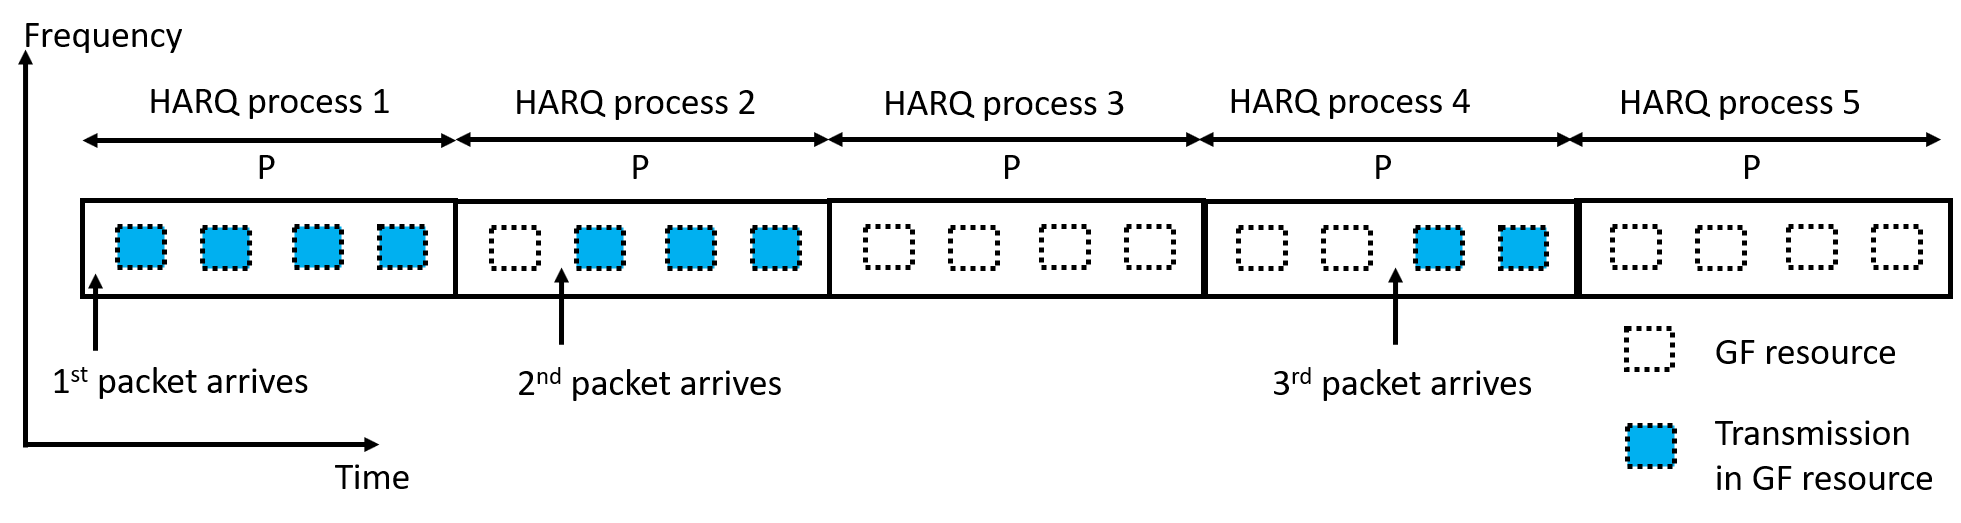
\includegraphics[scale=0.27]{fig16.png}}
\caption{Less than K repetitions in CG UL transmission.}
\label{fig20}
\end{figure}

It is evident that when the packet comes after the first CG occasions in a period, the UE transmits the packet with a smaller number than the number configured by repK. It degrades the reliability of UL transmission. The situation becomes more severe for the URLLC UEs with high reliability requirement. Moreover, latency of a transmission also increases because with a smaller number of repetitions, the gNB has a higher probability of failing to decode the packet and needs to schedule a retransmission. In that case, the UE needs to wait the gNB to decode the repetitions of the packet and transmit an UL grant to reschedule a retransmission if necessary and it has a huge impact on latency.

\subsubsection{Prior art}
In 3GPP Release 15, the only option for the UE is to wait until the next period to start the transmission and fulfill the configured number of repetitions. Nevertheless, this option causes big delay and prevents the UE from meeting the URLLC latency requirement, especially for low SCS. 

In \cite{ad17} and \cite{ad18}, repetitions are allowed to cross the boundary of a periodicity when the UE cannot make the requiring repetitions. This solution leads to a confusion of HARQ ID that makes the UE not differentiate the initial transmission and the retransmissions in order to combine and decode a specific codeblock. Besides that, a new mechanism needs to be defined to communicate explicitly HARQ ID from the UE to the gNB and results in overhead and effort in standardization.  

Multiple configurations in CG region are proposed in \cite{ad19} and \cite{ad20}. A UE is configured with configurations having different time offsets so it can choose the nearest configuration to start a transmission and guarantee the number of repetitions. The main concern of multiple configurations is the control overhead and delay because of signals used to configure the UE as well as resource consumption if resources in the configurations are not overlapped.

\cite{ad21} and \cite{ad22} propose to use shared resource for URLLC repetitions to improve resource utilization. However, they do not count a constraint that the UE cannot do repetitions crossing the border of a period. If this constraint is not solved, it might lead to a number of repetitions smaller than the configured number. In addition, shared resources are allocated periodically with the same size for all transmission occasions. These two drawbacks bring an increase of resource consumption and a drop of reliability.

In this work, an UL CG transmission scheme with reserved resources is described. Reserved resources are used and shared among the UEs when they need to transmit repetitions crossing the border of a transmission period P in order to achieve the target number of repetitions. These reserved resources have different sizes that are optimized based on the positions of their transmission occasions. 

Firstly, reserved resources and calculations to optimize their sizes are presented in Section \ref{C2}. The process allowing the UEs to access to these resources is also discussed. Section \ref{C3} shows numerical results obtaining from the equations derived in diverse scenarios. Finally, Section \ref{C4} provides the concluding remarks for this work.

\subsection{Strategy to ensure the configured number of repetitions in UL CG transmission}\label{C2}

\subsubsection{Reserved resources}\label{C21}

To make the URLLC UEs achieve the strict requirements, a strategy to ensure that the UEs can transmit the number of repetitions as configured by repK from higher layer is indispensable. Reserved periodic resources are proposed to be created and assigned to multiple UEs by the gNB so that they are likely to retransmit data in case the transmissions in the reserved resources are necessary to ensure the configured number of repetitions. These reserved resources have the same periodicity as the CG resources.

\begin{figure}[htbp]
\centerline{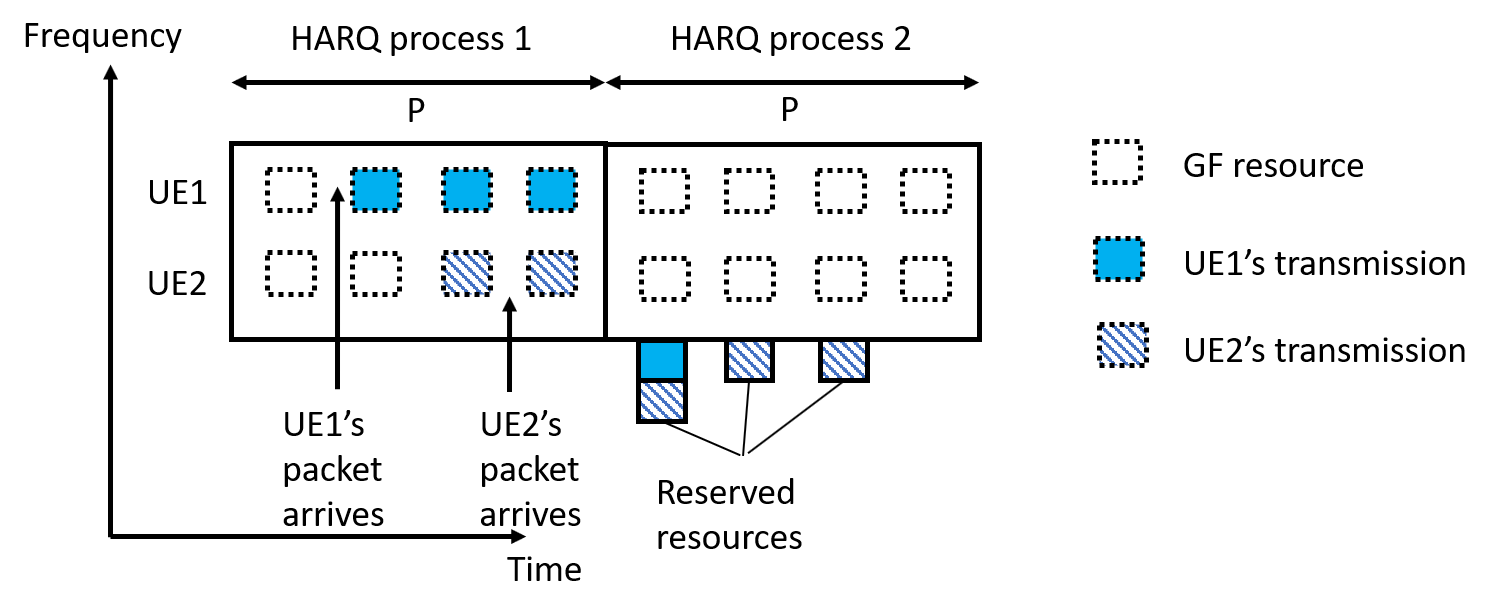
\includegraphics[scale=0.30]{fig17.png}}
\caption{Reserved resources for repetitions.}
\label{fig21}
\end{figure}

The use of reserved resources is shown in Fig.~\ref{fig21}. There are 2 UEs considered with CG resources in different bandwidth and each UE is configured with repK = 4. UE1's data comes after the first CG occasion in the first period so it only can do 3 repetitions in the period. In order to attain 4 repetitions, the UE1 retransmits data in the first reserved resource of the next period. Similarly, UE2's data arrives at the last CG occasion and only one repetition can be made. Thus, the UE2 uses the 3 reserved resources in the next period to achieve the configured number of repetitions.

In the example, 4 repetitions are configured so 3 reserved resources are needed in the next period. To increase the efficiency of resource consumption, the reserved resources are shared among the UEs. The first reserved resource in Fig.~\ref{fig21} with 2 blocks is likely to be shared with more than 2 UEs while still attain the target collision probability being approximate to the collision probability in the CG resources. Similarly, the second and third reserved resources are also shared by a group with more than 2 UEs. The equation showing the relation among the number of UEs, the size of the reserved resources and the collision probability is derived in Section \ref{C23}.

\subsubsection{System model}\label{C22}

\begin{figure}[htbp]
\centerline{
\includegraphics[scale=0.3]{fig18.png}}
\caption{UL transmission resources' distribution.}
\label{fig22}
\end{figure}

The system in Fig.~\ref{fig22} considered to calculate collision probability in the reserved resources contains $N$ UEs. These $N$ UEs are configured by the gNB to transmit in the periodical CG resources with the number of repetitions $K$ set by parameter repK. The UEs transmit the automatic repetitions of a packet in the consecutive CG resources. The CG resources in one frequency band can be shared among the UEs in a group. A period $P$ corresponding to a HARQ process consists of CG transmission occasions equal to the number of repetitions $K$. The results derived below are also valid if the number of CG transmission occasions in a period are bigger than $K$. The reserved resources ($K-1$ reserved resources) are configured periodically as CG resources in each period $P$. These resources are shared among the $N$ UEs to retransmit data in case the number of repetitions that they can carry out in one period are less than the configured one. Each reserved resource has size of $M_{i}$ blocks with index $i$ indicating that the reserved resource is at the $i$th transmission occasion of a period. The size of each block in the reserved resources is the same as that of the CG resource in one transmission occasion.

The arrival of data for each UE follows a Poisson process with the average number of random access events in an interval $\lambda$ calculated from the period between the CG resources $T$ and an average packet inter-arrival time $\mu$: $\lambda$ = $T/\mu$.

\subsubsection{Collision probability in reserved resources}\label{C23}

With random access, the $N$ UEs in system are allowed to use any block in the reserved resources of a specific transmission occasion if they need to do the transmissions in order to fulfill the configured number of repetitions.

The collision probability in the reserved resource at the first transmission occasion of a period (at t21 in Fig.~\ref{fig22}) is calculated as follow by considering 1 UE of interest having a transmission in the reserved resource at t21 and the rest of (N-1) UEs . 
In time $T$ between two CG resources, the probability that one UE has one or more random transmissions is \useshortskip

\begin{equation}
P_{data} = 1 - e^{-\lambda},\label{eq8}
\end{equation}

The CG resources in one bandwidth can be shared between a group of the UEs so collision probability in the CG resources between the UE of interest and other UEs of group is \useshortskip

\begin{equation}
P_{c\_CG} = 1 - e^{-\lambda(N_\mathrm{UE\_group}-1)},\label{eq9}
\end{equation}
where $N_\mathrm{UE\_group}$ is the number of the UEs that use the same frequency band of CG resources.

The reserved resource at t21 is used by a UE if its data comes after the first CG transmission occasion at t11. The probability that one UE has transmission after the first CG transmission occasion in a period $P$ is \useshortskip

\begin{equation}
P_{d} = 1 - (1-P_{data})^{K-1}.\label{eq10}
\end{equation}

There is no collision in the first reserved resource of a period $P$ at t21 if no UE rather than the UE of interest has a transmission after the first CG transmission occasion at t11. The probability that no other UE from the set of $N-1$ UEs has a transmission after the first CG occasion is calculated by \useshortskip

\begin{equation}
P_{0} = (1-P_{d})^{N-1}.\label{eq11}
\end{equation}

In case other UEs in a set of $N-1$ UEs has a transmission after the first CG occasion, the probability that $n$  UEs have such transmission is \useshortskip

\begin{equation}
P_{n} = \binom {N-1}{n}P_{d}^{n}(1-P_{d})^{N-1-n}.\label{eq12}
\end{equation}

The probability that the UE of interest and $n$ UEs do not access the same resource block in the first reserved resource at t21 is \useshortskip

\begin{equation}
P_{a0\_n} = (\frac {M_{1}-1}{M_{1}})^{n}.\label{eq13}
\end{equation}

The probability that the UE of interest does not collide with any other UE in the first reserved resource at t21 is calculated by \useshortskip

\begin{equation}
P_{sum} = \sum_{n=1}^{N-1} P_{n}P_{a0\_n}.\label{eq14}
\end{equation}

From \eqref{eq11} and \eqref{eq14}, the collision probability in the first reserved resource for the UE of interest is derived as \useshortskip

\begin{align}
P_{c1} &= 1 - P_{0} - P_{sum} \nonumber\\
 &= 1 - (\frac{M_{1}-1+e^{-\lambda(K-1)}}{M_{1}})^{N-1}.\label{eq15}
\end{align}

Based on the same calculating process, a general equation of collision probability for the reserved resource at any transmission occasion in a period can be derived as \useshortskip

\begin{equation}
P_{ci} = 1 - (\frac{M_{i}-1+e^{-\lambda(K-i)}}{M_{i}})^{N-1},\label{eq16}
\end{equation}
where
$i \in [1, K-1]$ is index indicating the position of the reserved resource based on the position of transmission occasion in a period.

\subsubsection{Optimization of reserved resource size}

From \eqref{eq16} with a set of parameters  $\lambda, N, K, i,$ and $P_{ci}$, the size of the reserved resources at any transmission occasion can be calculated. To guarantee the reliability of transmission in the reserved resources in comparison to that in the CG resources, the target probability $P_{ci}$ is chosen to be approximate to $P_{c\_CG}$ in \eqref{eq9}. If $P_{ci}$ is set to have the same value in all the reserved resources, the trend of reserved resources' size in terms of their positions in a period is: $M_1 > M_2 > M_3 > ... > M_{K-1}$. The size of the reserved resources to achieve a target probability decreases gradually from the first to the last reserved resource in a period. The design of the reserved resources following this decreasing trend instead of using the same size for all of the reserved resource brings an efficiency of resource consumption because the size is optimized particularly for each reserved resource.

\subsubsection{Group access to the reserved resources}

In group access approach, one UE is only allowed to access and uses a specific part of the reserved resource pre-configured by the gNB. One part of the reserved resource is assigned and shared among a group of the UEs. For example, the UE1-3 is only permitted to access the resource blocks as shown in Fig.~\ref{fig23}. On the other hand, other UE groups are also prohibited to access the resource blocks pre-configured to the UE1-3. 

\begin{figure}[htbp]
\centerline{
\includegraphics[scale=0.35]{fig23.png}}
\caption{Group access to the reserved resource.}
\label{fig23}
\end{figure}

For a group of the UEs accessing to a part of the reserved resources, the collision probability is calculated by \eqref{eq16} as random access approach. The size of the whole reserved resource in each transmission occasion is sum of all parts assigned to the UE groups to guarantee a target probability. 

Simulation in Section \ref{C3} shows that the sizes of the reserved resources for both random access and group access approach are the same to achieve an equal target probability. However, group access approach reduces the decoding burden in the gNB. To decode a retransmitted packet, the gNB only needs to search a part of the reserved resource instead of the entire reserved resource as random access approach. Thereby, power consumption and processing time drop dramatically. 

When two or more UEs of the same group having access to a part of the reserved resources have data coming at the same time and need to use the reserved resource for repetitions, they will compete for the same part of the reserved resources at the consecutive transmission occasions as show in Fig.~\ref{fig24}. The UE 1 and 2 have 3 repetitions and data coming after the first two CG occasions so they compete two times at both the first and second reserved resources with the arrangement in the blue circle.

\begin{figure}[tbp]
\centerline{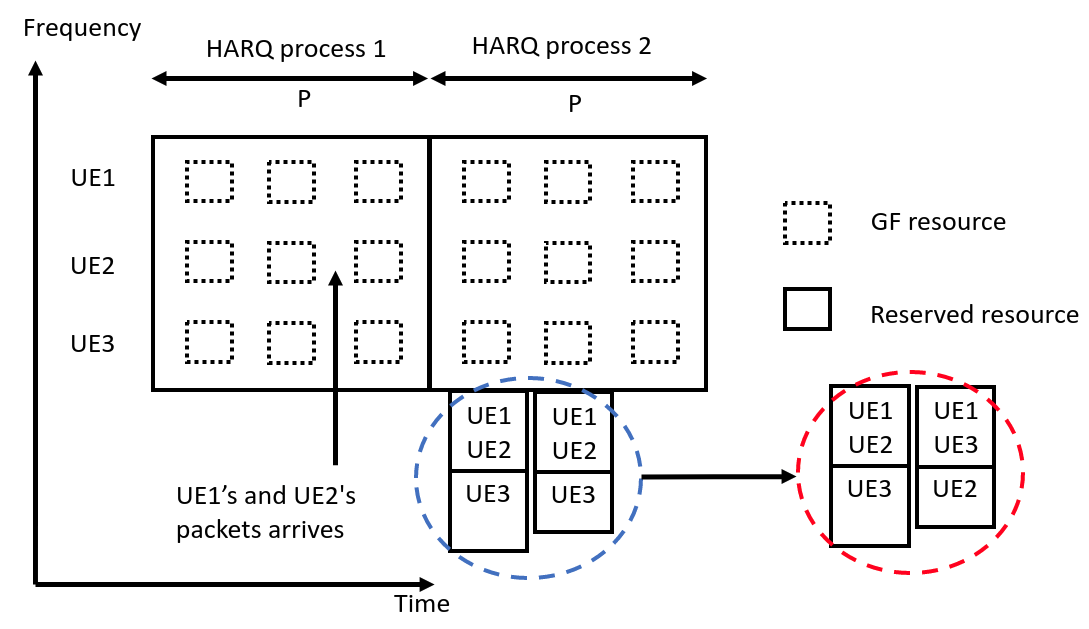
\includegraphics[scale=0.2]{fig24.png}}
\caption{Method to group the UEs in different transmission occasions.}
\label{fig24}
\end{figure}

To avoid that problem, the UEs are assigned to different groups of the reserved resources for different transmission occasions as illustrated in the red circle. The UE 1 only has the competition in both two reserved resources when both the UE 2 and 3 need to use the part of the reserved resources assigned to the UE 1 so the probability of having a competition decreases from $P_{data}$ to $P_{data}^2$ with $P_{data}$ calculated from \eqref{eq8}.

In each reserved resource, the collision probability is still the same as calculated from \eqref{eq16} but the overall reliability of a UE transmitting in the reserved resources at different transmission occasions will be improved with the hopping of the UEs to various groups in the different reserved resources.

\subsection{Numerical results and performance evaluation}\label{C3}

\subsubsection{Random access to the reserved resources}

From \eqref{eq16}, the number of the UEs that the system can support can be found. Besides, the number of resource blocks in each reserved resource are also calculated to sustain that system.

The simulation starts with the reserved resource in the first transmission occasion of a period. The set of parameters is $M_1=10, K=4, \lambda=1.25\times10^{-4}$.

Fig.~\ref{fig25}\subref{25a} shows collision probability in the reserved resource in the first transmission occasion in terms of the number of the UEs sharing that resource. From the graph, we see that if the target collision probability ($P_{c1}$) is 10\textsuperscript{-3}, the system can support 28 UEs in the first reserved resources.

\begin{figure}[htbp]
\centering
\subfloat[Collision probability with respect to the number of the UEs.\label{25a}]{%
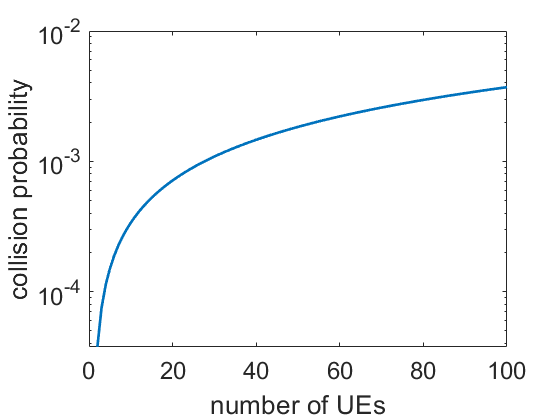
\includegraphics[scale=0.35]{fig19.png}}
\hspace{2em}
\qquad
\subfloat[Collision probability of the second reserved resource.\label{25b}]{%
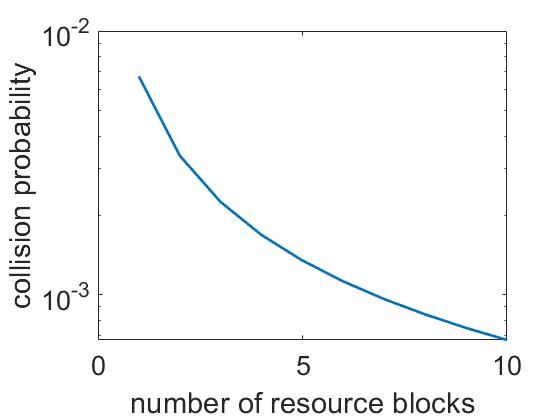
\includegraphics[scale=0.35]{fig20.png}}
\hspace{2em}
\caption{Collision probability.}
\label{fig25}
\end{figure}

As mentioned in Section \ref{C22}, the CG resources in a frequency band can be shared by a group of the UEs. 28 UEs calculated above can be divided in to 4 groups with 7 UEs in each group. The collision probability in the CG resources is $7.5\times10^{-4}$ that is approximate to the collision probability of 10\textsuperscript{-3} in the reserved resource.

When all the parameters ($\lambda, N, K$ and $P_{ci}$) are kept the same, the sizes of the reserved resources in the second and the third transmission occasions are calculated as shown in Table~\ref{tab8}.
%KHOA BEGIN
% THem ti khoang trong' duoi table, chon medskip, bigskip hoac smallskip
%\smallskip
%\smallskip
%\bigskip
\begin{table}[htbp]
\caption{Sizes of the reserved resources with $K=4$ and random access}
\begin{center}
\begin{tabular}{|p{10em}|p{2em}|p{2em}|p{2em}|}
 \hline
 \textbf{\textit{Position of reserved resources}} & $1$ &$2$ &$3$ \\ 
 \hline
 \textbf{\textit{Number of blocks}} & $10$ &$7$ &$3$ \\

%  increase row height, number of & = number of collumn
% &&&&&\\[-1em]
 
 \hline
\end{tabular}
\label{tab8}
\end{center}
\end{table}

%\medskip
%KHOA END

The percentage of resources saved in comparison to using the same size of 10 resource blocks for all the resources is: $(1 - (10+7+3)/(10\times3))\times100\% = 33\%$.

Fig.~\ref{fig25}\subref{25b} illustrates collision probability with respect to the reserved resource's size in the second transmission occasion.

Another scenario is considered with a bigger number of repetitions: $M_1=10, K=8, \lambda=1.25\times10^{-4}$ .

The system can support 12 UEs in the first reserved resources to achieve Pc target of 10\textsuperscript{-3}. These UEs can be divided into 2 groups with 6 UEs in one group that each group uses the CG resources in one bandwidth part. The collision probability in CG regions of a group of 6 UEs as scheduled above is: $6.25\times10^{-4}$.
With 12 UEs, the sizes of the reserved resources in the transmission occasions are shown in Table~\ref{tab9}.

\begin{table}[htbp]
\caption{Sizes of the reserved resources with $K=8$ and random access}
\begin{center}
\begin{tabular}{|p{5em}|p{2em}|p{2em}|p{2em}|p{2em}|p{2em}|p{2em}|p{2em}|}
 \hline
 \textbf{\textit{Position of reserved resources}} & $1$ &$2$ &$3$ & $4$ &$5$ &$6$ &$7$\\ 
 \hline
 \textbf{\textit{Number of blocks}} & $10$ &$8$ &$7$ & $6$ &$4$ &$3$ &$2$\\

%  increase row height, number of & = number of collumn
% &&&&&\\[-1em]
 
 \hline
\end{tabular}
\label{tab9}
\end{center}
\end{table}

The percentage of resources saved in comparison to using the same size of 10 resource blocks for all the resources is: $(1 - (10+8+7+6+4+3+2)/(10\times7)) \times100\% = 42.86\%$

As can be seen from two scenarios, the use of reserved resources with optimization from \eqref{eq16} brings an efficiency of resource utilization, especially for high configured number of repetitions. The resources needed are less than the approach of choosing blindly the same sizes for all reserved resources in different transmission occasions while still guarantees the number of repetitions with a target reliability.

Moreover, in the conventional scheme in 3GPP Release 15, the UE needs to wait until the next period if it cannot do the configured number of repetitions in the current period to fulfill the reliability requirement. Therefore, with $K=4$ and 4 transmission occasions in a period, in the worst case, the UE must wait 3 transmission occasions equal to 3 slots or 0.75ms with SCS 60kHz. This latency is close to the URLLC requirement of 1ms and causes the UEs not be able to make 4 repetitions as configured in the next period. In comparison, the proposed scheme allows the UE to start the transmission immediately and reach the configured number of repetitions in target latency of 1ms (4 repetitions consume 1ms with SCS 60kHz) as well as meet the reliability requirement.

\subsubsection{Group access to the reserved resources}

Group access is simulated with the parameters as the first scenario in random access: $N = 28, K = 4, \lambda = 1.25\times10^{-4}$.

28 UEs are divided into 4 groups of 7 UEs to access the reserved resources. Each group is only allowed to access the part of the reserved resources pre-configured to them. 

To satisfy Pc=10\textsuperscript{-3}, the sizes of the reserved resources are shown in Table~\ref{tab10}.

\begin{table}[htbp]
\caption{Sizes of the reserved resources with K=4 and group access}
\begin{center}
\begin{tabular}{|p{14em}|p{2em}|p{2em}|p{2em}|}
 \hline
 \textbf{\textit{Position of reserved resources}} & $1$ &$2$ &$3$ \\ 
 \hline
 \textbf{\textit{Number of blocks per group of reserved resources}} & $2$ &$2$ &$1$ \\
 \hline
\textbf{\textit{Total number of blocks of reserved resources}} & $8$ &$8$ &$4$ \\
%  increase row height, number of & = number of collumn
% &&&&&\\[-1em]
 
 \hline
\end{tabular}
\label{tab10}
\end{center}

\end{table}

The resource consumption is equal for random access and group access to the reserved resources as shown in Table~\ref{tab8} and Table~\ref{tab10}. However, with group access, the complexity and processing time of decoding in the gNB reduce substantially because in the reserved resource at the first transmission occasion, the gNB only needs to find data of a UE in 2 reserved blocks instead of finding blindly data of a UE in 10 reserved blocks as in random access approach.

\subsection{Conclusion}\label{C4}

This paper presents an approach with reserved resources shared among the UEs that allows them to carry out repetitions and reach the configured number so that reliability and latency requirements can be  satisfied. Each reserved resource has an optimized size to balance reliability and  resource consumption. 

\section{Improving reliability-latency in less than K repetitions UL transmission by flexibly moving to explicit HARQ feedback structure or transmitting an additional SR}\label{Ap4}

\subsection{Introduction}

The advent of new applications such as remote surgery, vehicle-to-everything communication, etc. with high demands of latency and reliability requires that 5G supports URLLC. The strict requirements of URLLC are given in \cite{ad1}: ``A general URLLC reliability requirement for one transmission of a packet is 10\textsuperscript{-5} for 32 bytes with a user plane latency of 1 ms''. These requirements continue to rise in the recent meetings of the 3rd Generation Partnership  Project  (3GPP): ``Higher reliability (up to 10\textsuperscript{-6}), higher availability, short latency in the order of 0.5 to 1 ms, depending on the use cases (factory automation, transport industry and electrical power distribution)''\cite{ad2}.

\subsubsection{Techniques accepted in 3GPP Release 15}\label{D11}
In order to facilitate the implementation of URLLC, 3GPP made three important decisions about physical layer design.

One of the aspects is a permission to use larger subcarrier spacings (SCS). In 5G, SCS is allowed to have a value up to 240 kHz instead of an unique value of 15 kHz as in LTE \cite{ad6}. The next aspect is about mini-slot based transmission that allows a UE to be scheduled in a period of one or several symbols rather than a whole slot \cite{ad7}. These two decisions bring down time alignment of arriving packets.

The third aspect is related to the UL transmission in CG region to lessen time consumption of SR and UL grant\cite{ad3}.

\subsubsection{Repetition problem in URLLC CG UL transmission}\label{D12}

As mentioned in Section \ref{D11}, in UL transmission, the base station (called gNB) can configure a set of CG resources to one or more UEs with a periodicity defined by parameters in Radio Resource Control (RRC) from higher layer. When a UE is configured to transmit in CG resources, it can transmit data immediately instead of sending SR and waiting for UL grant as grant-based (GB) transmission.

To further reduce latency as well as increase reliability of the transmission, the URLLC UEs transmitting in the CG regions are also configured to transmit automatically a number of repetitions (called $K$ repetitions with $K \in \{1, 2, 4, 8\}$ \cite{ad16}) defined by a parameter repK from higher layer instead of waiting an UL grant to reschedule data if necessary after each repetition. Nevertheless, the UEs are only permitted to carry out the repetitions in one HARQ process with a periodicity $P$ as shown in Fig.~\ref{fig27} (a set of allowed periodicities $P$ are defined in \cite{ad16}). Thereby, the UEs stop to do the repetitions at the boundary of a HARQ process even if they still do not reach the configured number of repetitions. In Fig.~\ref{fig27}, an interval $P$ contains 4 CG occasions, the UE is configured to do 4 repetitions. In the first period, data comes before all the 4 CG occasions so the UE is able to do 4 repetitions for the first packet as configured. However, when data comes in the second period, there are only 3 CG occasions left in that period. This means that the UE only can carry out 3 repetitions that are less than the configured number. Similarly, in the fourth period, the UE only can transmit the packet 2 times. 
\begin{figure}[htbp]
\centerline{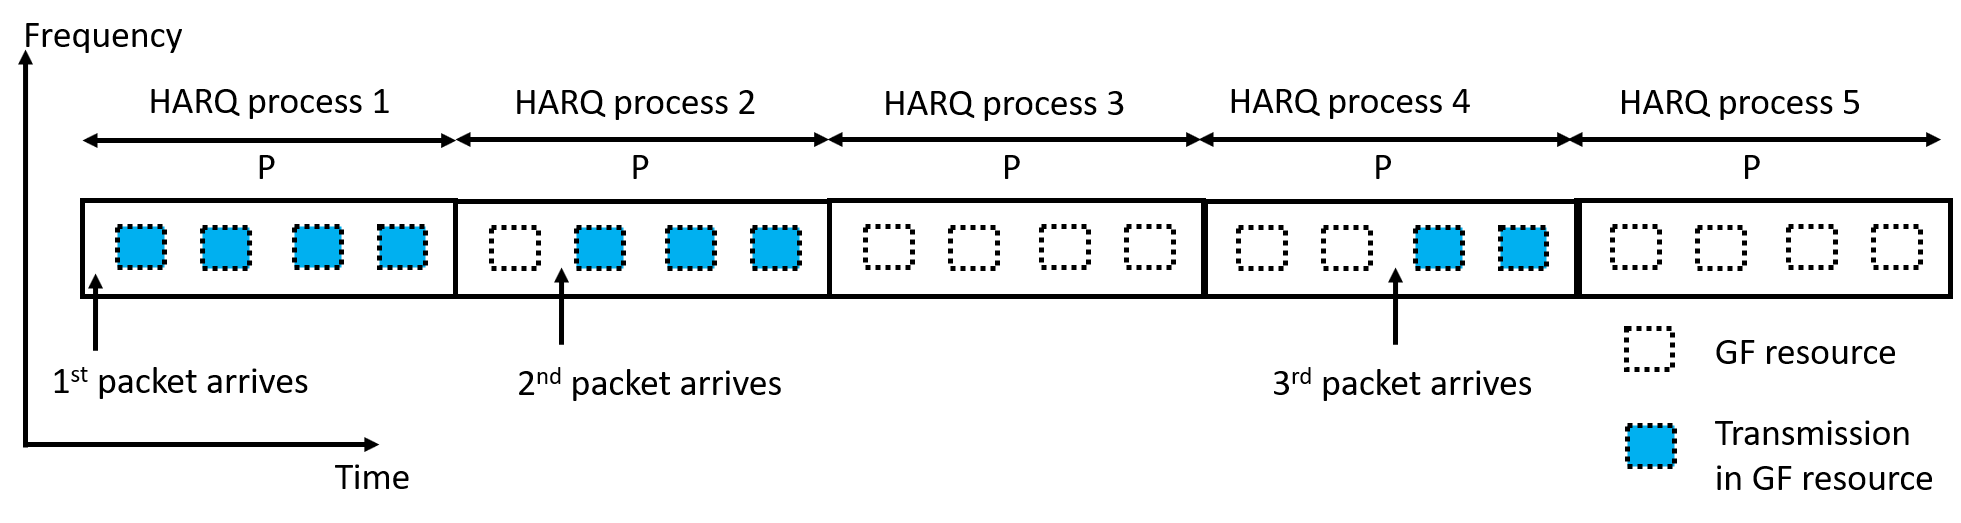
\includegraphics[scale=0.25]{fig16.png}}
\caption{Less than K repetitions in CG UL transmission.}
\label{fig27}
\end{figure}

This constraint is to help the gNB avoid a confusion in HARQ IDs of different HARQ processes that preventing its from recognizing the first repetition to do soft combining or determining the UE IDs to send an UL grant. However, this constraint also makes the system face a degradation of UL transmission's performance due to a smaller number of repetitions that is catastrophic to the URLLC UEs with high reliability requirement. It also impacts latency when the gNB cannot decode the packet because the configured number of repetitions are not transmitted, it must schedule a retransmission by an UL grant and the UE only carries out more retransmissions after receiving this UL grant.

\subsubsection{Prior art}
In 3GPP Release 15, an option for the UE is to wait until the next HARQ process to transmit the whole K repetitions if it cannot make K repetitions as configured in the current process because data comes late. This method leads to huge latency and might not suitable for URLLC.

In \cite{ad17} and \cite{ad18}, the UE does not stop at the boundary of a period $P$ if the configured number of repetions have not been reached. The UE is allowed to continue to transmit the repetitions across the boundary and only stops after transmitting all K repetitions. To avoid a confusion of HARQ ID as mentioned in Section \ref{D12}, a new mechanism needs to be defined to communicate explicitly HARQ ID from the UE to the gNB and results in big overhead and effort in standardization.  

Multiple configurations in CG region are proposed in \cite{ad19} and \cite{ad20}. A UE is configured with configurations having different starting time offsets so it can choose the nearest configuration to start a transmission without having to wait long time until the next period and guarantee the number of repetitions. However, this method causes big overhead from downlink control information (DCI) used to configure different configurations to the UEs. Resource consumption is another concern, if the configurations are configured separately without any overlap. 

\cite{ad21} and \cite{ad22} propose to use shared resource for URLLC repetitions to improve resource utilization. However, they do not count a constraint that the UE cannot do repetitions crossing the border of a period. If this constraint is not solved, it might lead to a number of repetitions smaller than the  number configured and transmission reliability is degraded.

In this work, two methods are presented to enhance the performance of URLLC UL CG transmission in case the UE cannot make K repetitions as configured. The first method described in Section \ref{D2} applies an explicit HARQ feedback structure to the transmisisons with less than K repetitions. The second method in Section \ref{D3} asks the UEs with less than K repetition to transmit a SR in parallel with data packet. These two methods guarantee a retransmission in case of DMRS miss-detection due to a smaller number of repetitions. Section \ref{D4} shows numerical results and performance evaluation. Finally, Section \ref{D5} provides the concluding remarks.

\subsection{Improving reliability-latency by flexibly moving to explicit HARQ Feedback structure}\label{D2}

\subsubsection{Operation of explicit HARQ feedback structure}

The HARQ structure in UL CG transmission is timer-based. This means that there is no explicit acknowledgement (ACK) feedback sent from the gNB to the UE if data is decoded correctly. Instead, the UE uses a timer. If it does not receive an UL grant to schedule a retransmission at the end of time configured in the timer, the transmission is considered as successful. This structure has a drawback because the UE cannot differentiate between a successful transmission and a miss-detection when the gNB cannot decode DMRS to identify the UE and transmits UL grant. Therefore, in case of miss-detection, the UE does not receive any signal from the gNB, it assumes a successful transmission and drops data in buffer. This behavior impacts reliability of a transmission and becomes more severe in less-than-K-repetitions situation. Once the UE is not able to carry the configured number of repetitions, the QoS of transmission is badly affected and there is a higher probability that the gNB cannot decode DMRS sequence. It leads to a degradation of URLLC transmission due to packet dropped by the UE. To handle the issue with CG transmissions with less than K repetitions, we propose to use explicit HARQ feedback from the gNB. 

An UL transmission results in three scenarios: one for correct decoding and two scenarios for incorrect decoding. In explicit HARQ feedback structure, the UE's behavior in each scenario will be analyzed as follows. 

The first scenario is about correct data decoding. The gNB tries to combine all the repetitions of a TB to facilitate data decoding, and the number of these repetitions can be less than K as per the previous discussion. For a normal operation, the gNB is capable of identifying the repetitions concerning a specific TB. Thus, whenever the gNB is able to correctly decode a TB, and it sees that it was sent with less than K repetitions, it will send an explicit ACK for this TB to the transmitting UE.

The second scenario is about a failure of data decoding with a successful UE identification. When the UE transmits less than K repetitions, it is possible that the data decoding is not successful but the gNB is able to identify the UE transmitting the TB with less than K repetitions through identification of UE specific DMRS sequence which it was configured with as part of CG configuration. In this case, the gNB will reschedule a retransmission of the previously transmitted TB. 

The third scenario is related to UE identification failure. It is where the proposed explicit feedback becomes pivotal. The bad quality of received data may lead to a situation when the gNB is unable to identify the transmitting UE. This situation is the most damaging for the URLLC UEs/applications due to their tight constraints on latency and reliability. With a timer-based HARQ structure, which is currently used for URLLC transmissions in 3GPP Release 15, this situation leads to different understanding at the gNB and at the UE. The gNB, being unable to identify the UE, cannot schedule the re-transmission. The UE, upon receiving no UL grant for re-transmission, considers the packet successfully decoded at the gNB and discards the buffer upon the expiry of HARQ timer.

Although the situation when the gNB cannot identify the UE may be caused by a number of reasons such as the very bad channel conditions, large amount of interference or insufficient number of actual repetitions, the configuration parameters of CG transmission, in particular MCS and the number of repetitions K, are designed to combat most of these adverse effects. On the other hand, if the configured number of repetitions cannot be made, this brings the CG operation point to a lower QoS target than the desired operating point.

In the proposed technique, whenever the UE transmits less than K repetitions, the TB in question is supposed to operate with explicit HARQ based feedback. In general, the gNB can identify transmissions with less than K repetitions thanks to DMRS detection and CG window boundary knowledge. When the gNB fails to identify the transmitting UE and sends no ACK or UL grant to this UE, the UE upon expiry of configured HARQ timer re-transmits automatically the TB. 

The retransmission timing and resources can be configured as part of the explicit HARQ feedback configuration. One suitable option is to retransmit in the closest CG periodic window after the expiry of HARQ feedback timer. The HARQ feedback timer should include the time for the gNB to decode the data and find the suitable occasion for potential DL transmission of HARQ ACK or UL grant.

\subsubsection{Design of explicit HARQ feedback}

In the proposed strategy, the UEs are allowed to request explicit HARQ feedback for certain TBs. Thus, a design for the explicit HARQ feedback in general may be needed. One strategy can be to define a channel where HARQ ACK can be transmitted. This can be similar to Physical HARQ Indicator Channel (PHICH) as specified in 4G LTE but this requires a lot of specification effort and high resource overhead. The rationale is that in typical operation mode, the UEs will not request explicit HARQ feedback to reduce overhead and only in exceptional cases it will be required. 

With this in view, the proposal is to use the UL grant (which is DCI) as an explicit HARQ feedback. This DCI can be sent with UE specific configured scheduling-radio network temporary identifier (CS-RNTI) which is used with configured GB transmissions. If the gNB is able to successfully decode the data, it sends DCI to this UE with the same HARQ process number (HARQ ID) as of the successfully received TB. To avoid any confusion between DCI used as feedback and DCI used as UL grant, new data indicator (NDI) field can be set to 0. Further, some of the fields in the DCI such as the time and frequency resource assignment fields are set to 0 to help the UE differentiate two types of DCI.

\subsection{Improving reliability-latency by flexibly transmitting an additional Scheduling Request }\label{D3}

In this section, another scheme is proposed to deal with the problem of less-than-K repetitions. In this scheme to improve the reliability of UL CG transmissions, whenever the UE transmits less than the configured number of repetitions for a TB, it sends SR to the gNB, in parallel to transmission of TB with less than K repetitions. This SR provides a sort of diversity mechanism in parallel to the transmission of the TB.

3GPP Release 15 does not allow transmission of Physical uplink control channel (PUCCH) and Physical uplink shared channel (PUSCH) simultaneously. The UE transmits UCI encoding SR, HARQ feedback, etc on PUCCH. Therefore, the UE multiplexes UCI and PUSCH if it wants to transmit uplink control information (UCI) while sending PUSCH. This strategy allows the UE to transmit SR in case of less than K repetitions. However, in UCI and PUSCH  multiplexing, if the gNB cannot detect DMRS of PUSCH due to bad channel, there is high probability that the gNB also cannot decode UCI (SR) to find the UE ID. Thus, multiplexing strategy might not enhance the performance of UE ID detection. For this reason, SR should be configured to be transmitted on the configured PUCCH resources. The gNB upon receiving PUCCH and PUSCH from the same UE will understand that the SR in PUCCH is for the same TB sent in PUSCH for the UE that is only able to make less than K repetitions.

Table~\ref{tab15} shows in tabular format the UE and gNB actions for strategy of SR transmission in parallel to TB transmission. 

\begin{table}[htbp]
\caption{SR Transmission with TB and Actions for the gNB and the UE}
\begin{center}
\begin{tabular}{|p{2em}|p{6em}|p{7em}|p{9em}|p{8em}|p{8em}|}
 \hline
 \textbf{Case} & \textbf{CG PUSCH} & \textbf{SR in PUCCH} & \textbf{gNB understanding} & \textbf{gNB action} & \textbf{UE action}\\ 
 \hline
 1 & Correctly decoded at the gNB & Correctly decoded at the gNB & The gNB knows that SR is for the decoded TB & Indicate a correct detection (ex: using UL grant with the same HARQ ID) & Discard data upon receiving the gNB indication\\
 \hline
 2 &  Correctly decoded at the gNB & Incorrectly decoded at the gNB & The gNB upon correctly decoding the data and seeing less than K rep knows about missing SR. This case should be rare as SR is sent with strong coding & Indicate correct detection (ex: using UL grant with same HARQ ID) & Discard the data upon the gNB indication\\
\hline
3 & Incorrectly decoded at the gNB but UE Identified through DMRS & Correctly decoded at the gNB & the gNB understands that UE sent SR along with the TB that it failed to decode & The gNB sends the UL grant for re-transmission & The UE follows the UL grant for re-transmission\\
\hline
4 & Incorrectly decoded and UE Identification Failure at the gNB & Correctly decoded at the gNB & The gNB completely misses the CG transmission due to failure in UE identification but it receives SR. From the timing of SR and CG configurations, the gNB knows its decoding failure & The gNB sends the UL grant for transmission & The UE follows the UL grant for transmission and re-transmits the data\\
\hline
5 & Incorrectly decoded at the gNB but UE Identified through DMRS & Incorrectly decoded at the gNB & The gNB identifies the UE from PUSCH. If it can identify the case of less than K repetitions, it knows also about SR detection failure & The gNB sends the UL grant for re-transmission & The UE follows the UL grant for re-transmission\\
\hline
 6 & Incorrectly decoded at the gNB and UE Identification Failure at the gNB & Incorrectly decoded at the gNB & The gNB has no indication about UE transmission & No action & The UE can be configured to
retransmit in the subsequent CG resources or SR\\
 

%  increase row height, number of & = number of collumn
% &&&&&\\[-1em]
 
 \hline
\end{tabular}
\label{tab15}
\end{center}
\end{table}

The parallel transmission of PUCCH and PUSCH maybe slightly onerous for certain UEs because the UEs need to create the gap in the resource grid between PUCCH and PUSCH to protect them from interfernce. Nevertheless, considering that the main focus is here on URLLC type of UEs with strict latency and reliability targets, this overhead may be acceptable.

If the UE is transmitting different types of traffic at the same time, the gNB can differentiate the proposed SR transmitted in parallel with PUSCH in CG resources from a standalone classic SR which is sent to the gNB to have the UL resources scheduled through the HARQ ID of the transmitted TB included in the SR. As upon receiving the TB, the gNB will know its HARQ ID from its timing window, it will be able to conclude that the SR concerns the same TB or not.

Under certain situations, it may be beneficial to allow a hybrid scheme where the UEs can flexibly choose between an explicit HARQ feedback structure or sending an SR in parallel to the transmission of the transport block, when they are able to make less than K repetitions. The simplest scheme would be the one that the gNB configures the UEs to follow one of these two schemes. Alternatively, the UEs can be configured to choose one these two schemes. In that case, it would make sense to have an explicit indication in the TB for the explicit HARQ feedback. If the UEs choose to transmit SR in parallel to the transmission of the TB, they do not trigger explicit feedback with the TB transmission. This can be advantageous in the situations when there is at least a suitable SR transmission occasion available where the UEs can transmit SR for the TB in question. In the contrary situation, the UEs do not transmit SR in parallel to the transmission of the TB but send an indication to trigger explicit HARQ feedback. This can be more advantageous if for example, there is no suitable SR transmission occasion and a transmission of SR may harm the latency budget.

For the traffic with extremely stringent latency-reliability constraints, it can be foreseen that both mechanisms, explicit HARQ feedback and transmission of SR, are triggered in parallel to maximize the reliability within a short time interval when the UE transmits the TB with less than K repetitions.

\subsection{Numerical results and performance evaluation}\label{D4}

\begin{table}[htbp]
\caption{Simulation parameters}
\begin{center}
\begin{tabular}{|p{8em}|p{8em}|}
 \hline
 \textbf{Parameters} & \textbf{Values}\\
 \hline
 Waveform & CP-OFDM\\
 \hline
 Subcarrier spacing & 60kHz\\
 \hline
 Channel model & Rician\\
 \hline
 K factor & 1\\
 \hline
 Number of allocated PRB & 8\\
 \hline
 DMRS detection mechanism & Time-domain correlation\\
 

%  increase row height, number of & = number of collumn
% &&&&&\\[-1em]
 
 \hline
\end{tabular}
\label{tab16}
\end{center}

\end{table}

\begin{figure}[htbp]
\centerline{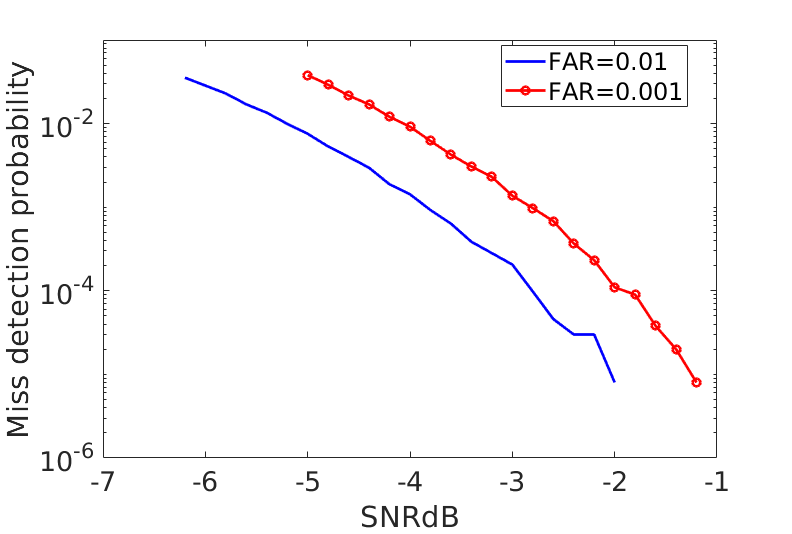
\includegraphics[scale=0.3]{fig26.png}}
\caption{DMRS detection performance.}
\label{fig28}
\end{figure}

Simulation parameters for the performance of DMRS detection of each repetition in Fig.~\ref{fig28} are shown in Table~\ref{tab16}. For each DMRS detection, the correlation result is compared with a threshold to determine whether DMRS exists or not. This threshold is chosen according to a target false alarm rate (FAR) indicating the cases that the gNB determines the existence of DMRS while in reality there is no DMRS transmitted. A higher threshold is required for a lower FAR but also results in more missed detection. As DMRS dectection is mandatory for channel estimation to decode data as well as for recognizing UE ID to reschedule a retransmission if necessary in conventional scheme, a degradation of DMRS detection due to a smaller number of repetitions than configured makes the system not be able to support reliability URLLC requirement.

\begin{table}[htbp]
\caption{Performance comparison of different schemes when data comes after the first occasion in a period at $SNR = -5dB$ and $FAR = 0.001$}
\begin{center}
\begin{tabular}{|p{6em}|p{4em}|p{4em}|p{4em}|p{4em}|p{4em}|}
 \hline
 \textbf{Case} & \textbf{Starting time offset (ms)}&\textbf{Number of repetitions}&\textbf{UE ID miss-detection probability}&\textbf{Retrans in ID miss-detection}&\textbf{Total UE ID miss-detection probability}\\
 \hline
 Conventional transmission&$0$&$3$&$5.5\times10\textsuperscript{-5}$&$0$&$5.5\times10\textsuperscript{-5}$\\
 \hline
 Conventional transmission with the UE waiting the next period&$0.75$&$1$&$0.038$&$0$&$0.038$\\
 \hline
Transmission with explicit ACK&$0$&$3$&$5.5\times10\textsuperscript{-5}$&$1$&$2.1\times10\textsuperscript{-6}$\\
\hline
Transmission with SR&$0$&$3$&$2.1\times10\textsuperscript{-6}$&$0$&$2.1\times10\textsuperscript{-6}$\\
 \hline
\end{tabular}
\label{tab17}
\end{center}
\end{table}

\begin{table}[htbp]
\caption{Performance comparison of different schemes when data comes after the second occasion in a period at $SNR = -5dB$ and $FAR = 0.001$}
\begin{center}
\begin{tabular}{|p{6em}|p{4em}|p{4em}|p{4em}|p{4em}|p{4em}|}
 \hline
 \textbf{Case} & \textbf{Starting time offset (ms)}&\textbf{Number of repetitions}&\textbf{UE ID miss-detection probability}&\textbf{Retrans in ID miss-detection}&\textbf{Total UE ID miss-detection probability}\\
 \hline
 Conventional transmission&$0$&$2$&$10\textsuperscript{-3}$&$0$&$10\textsuperscript{-3}$\\
 \hline
 Conventional transmission with the UE waiting the next period&$0.5$&$2$&$10\textsuperscript{-3}$&$0$&$10\textsuperscript{-3}$\\
 \hline
Transmission with explicit ACK&$0$&$2$&$10\textsuperscript{-3}$&$2$&$2.1\times10\textsuperscript{-6}$\\
\hline
Transmission with SR&$0$&$2$&$5.5\times10\textsuperscript{-5}$&$0$&$5.5\times10\textsuperscript{-5}$\\
 \hline
\end{tabular}
\label{tab18}
\end{center}
\end{table}

\begin{table}[htbp]
\caption{Performance comparison of different schemes when data comes after the third occasion in a period at $SNR = -5dB$ and $FAR = 0.001$}
\begin{center}
\begin{tabular}{|p{6em}|p{4em}|p{4em}|p{4em}|p{4em}|p{4em}|}
 \hline
 \textbf{Case} & \textbf{Starting time offset (ms)}&\textbf{Number of repetitions}&\textbf{UE ID miss-detection probability}&\textbf{Retrans in ID miss-detection}&\textbf{Total UE ID miss-detection probability}\\
 \hline
 Conventional transmission&$0$&$1$&$0.038$&$0$&$0.038$\\
 \hline
  Conventional transmission with the UE waiting the next period&$0.25$&$3$&$5.5\times10\textsuperscript{-5}$&$0$&$5.5\times10\textsuperscript{-5}$\\
 \hline
Transmission with explicit ACK&$0$&$1$&$0.038$&$3$&$2.1\times10\textsuperscript{-6}$\\
\hline
Transmission with SR&$0$&$1$&$10\textsuperscript{-3}$&$0$&$10\textsuperscript{-3}$\\
 \hline
\end{tabular}
\label{tab19}
\end{center}
\end{table}

In considered system, periodicity $P$ of HARQ process is 4 slots spreading in 1ms with SCS of 60kHz. The UE is configured to transmit 4 repetitions. As specified in \cite{ad6}, each slot only contains one repetition so one repetition consumes 0.25ms and the UE needs 4 slots to carry out all 4 configured repetitions and satisfies URLLC latency budget of 1ms.

Table~\ref{tab17}, Table~\ref{tab18} and Table~\ref{tab19} show the performance of DMRS detection at SNR of -5dB and FAR of 0.001 in various schemes and arrival time of data. As can be seen with conventional  transmission, due to the constraint of boundary of a period $P$, the UE cannot transmit 4 configured repetitions and it affects DMRS detection's performance. The later the packet comes, the worse DMRS detection is. In the timer-based feedback of the conventional scheme, the packet is lost because the UE assumes a successful transmission in case of DMRS miss-dection. Even if the UE waits for the next period with the intention of carrying of K repetitions configured as the second scheme, it also cannot achieve that intention because of URLLC latency requirement of 1ms. The more time the UE waits, the less time it has to transmit the repetitions. In consequence, it also cannot transmit K repetitions and DMRS miss-detection grows.

The presence of explicit feedback solves the problem of an increase of DMRS-miss detection because it helps the UE differentiate between a successful transmission and DMRS-miss detection. Therefore, the UE is able to retransmit packet even if the gNB does not detect UE ID by DMRS detection and reliability is guaranteed (total miss-detection probability of $2.1\times10\textsuperscript{-6}$ smaller than the conventional schemes) as shown in Table~\ref{tab17}, Table~\ref{tab18} and Table~\ref{tab19}.

These three tables also show that an additional SR transmitted in parallel with data provides another chance for the gNB to identify the UE and compensates for the missing repetitions due to boundary constraint so system performance is enhanced. 

The usages of an explicit feedback or an additional SR increase resource consumption. However, these approaches are only used in the critical situation as less than K repetitions made by the UE so a growth of resource consumption is limited. In addition, in case of less than K repetitions, the URLLC performance is degraded. Regarding the priorities of latency and reliability, resources used for the explicit feedback or the SR are necessary to guarantee those strict requirements.

\subsection{Conclusion}\label{D5}

In URLLC CG UL transmission. a packet is configured with K repetitions to achieve target QoS. However, because of boundary of a period P and arrival time of data, the UEs are only able to transmit less than K repetitions so the target QoS is not attained. This paper presents two strategies to help the UEs achieve the target QoS in case of less than K repetitions. These approaches relating to an explicit HARQ strucutre and an additional SR can be used individually or combined together based different scenarios. The results show that they improve the UE ID detection at the gNB.

\end{comment}
\end{document}
